Postoje dvije vrste podataka na kojima je moguće provesti ovo istraživanje: slika i video. Nije potrebno navoditi da koristeći sliku, zbog svojstva statičnosti, eliminiramo zadatak praćenja objekata.

\section{Viola-Jones algoritam}

Algoritam Viole i Jones-a, iako osmišljen davno, koristi se i danas. Izuzetno je brz, dovoljno točan i zahtjeva malo računalnih resursa. Sami algoritam opisan je u poglavlju 3.2. 

\begin{figure}[htp]
	\centering
	\begin{subfigure}[b]{0.4\linewidth}
		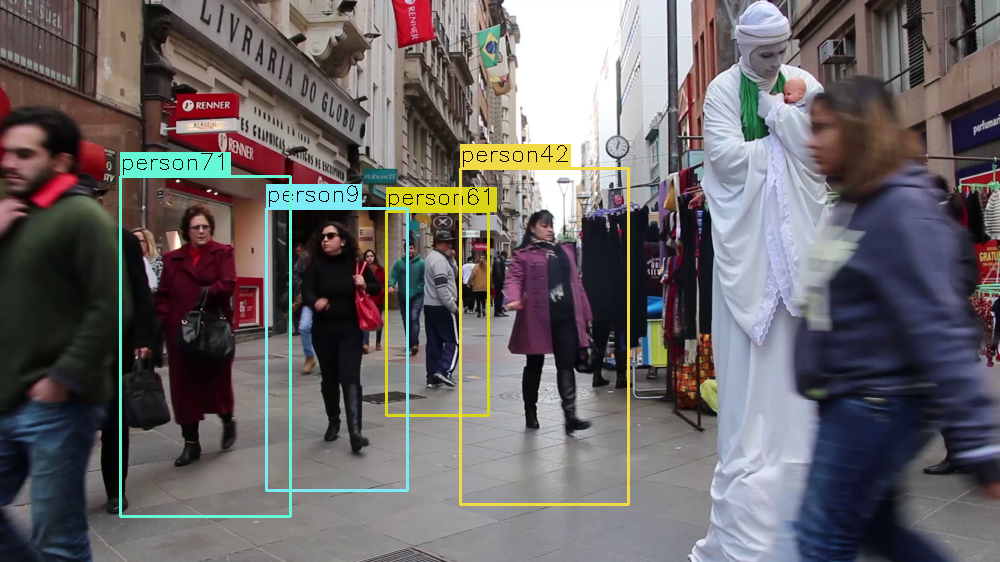
\includegraphics[width=\linewidth]{/home/luka/Workspaces/diplomski-rad/img/frame_0.png}
	\end{subfigure}
	\begin{subfigure}[b]{0.4\linewidth}
		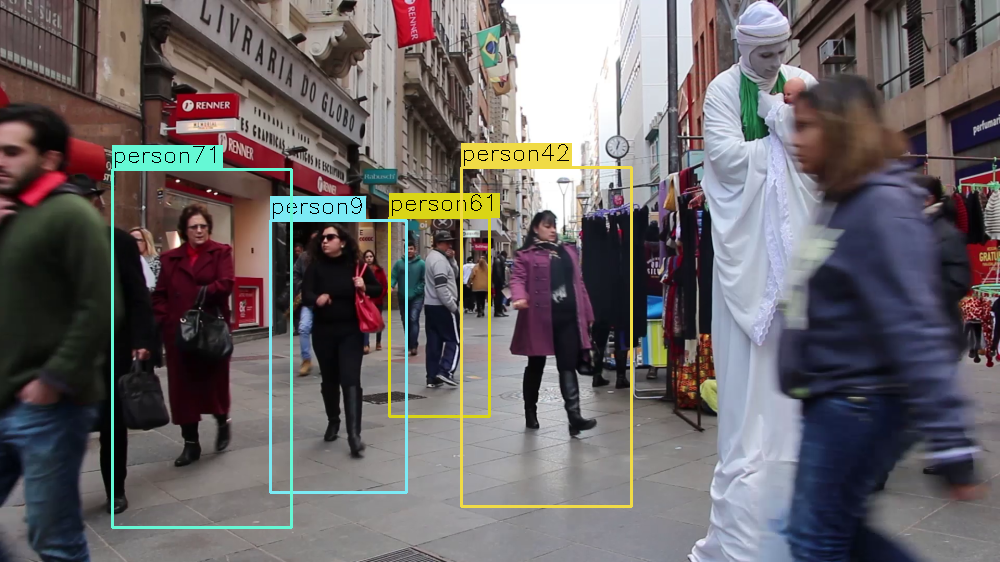
\includegraphics[width=\linewidth]{/home/luka/Workspaces/diplomski-rad/img/frame_1.png}
	\end{subfigure}
	\begin{subfigure}[b]{0.4\linewidth}
		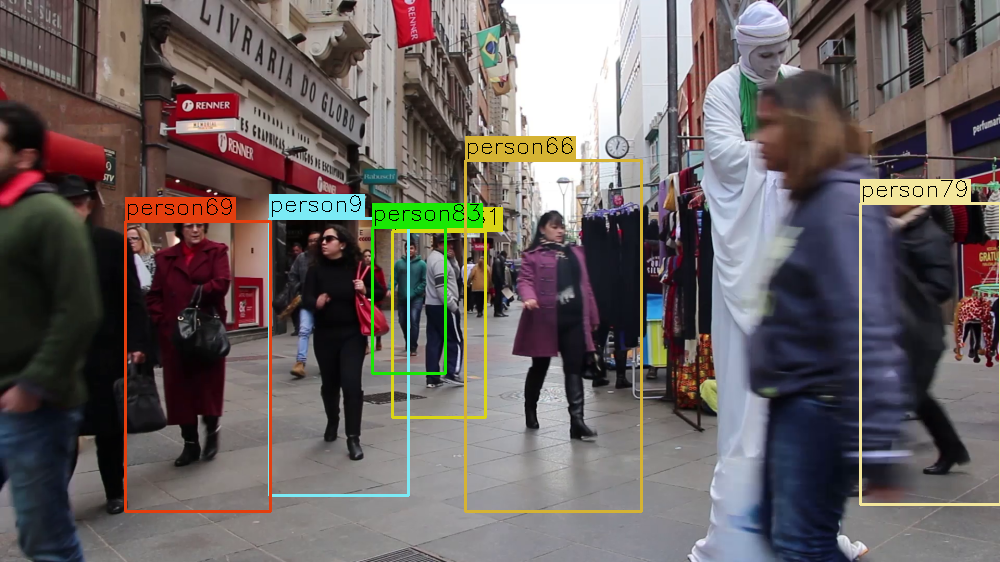
\includegraphics[width=\linewidth]{/home/luka/Workspaces/diplomski-rad/img/frame_3.png}
	\end{subfigure}
	\begin{subfigure}[b]{0.4\linewidth}
		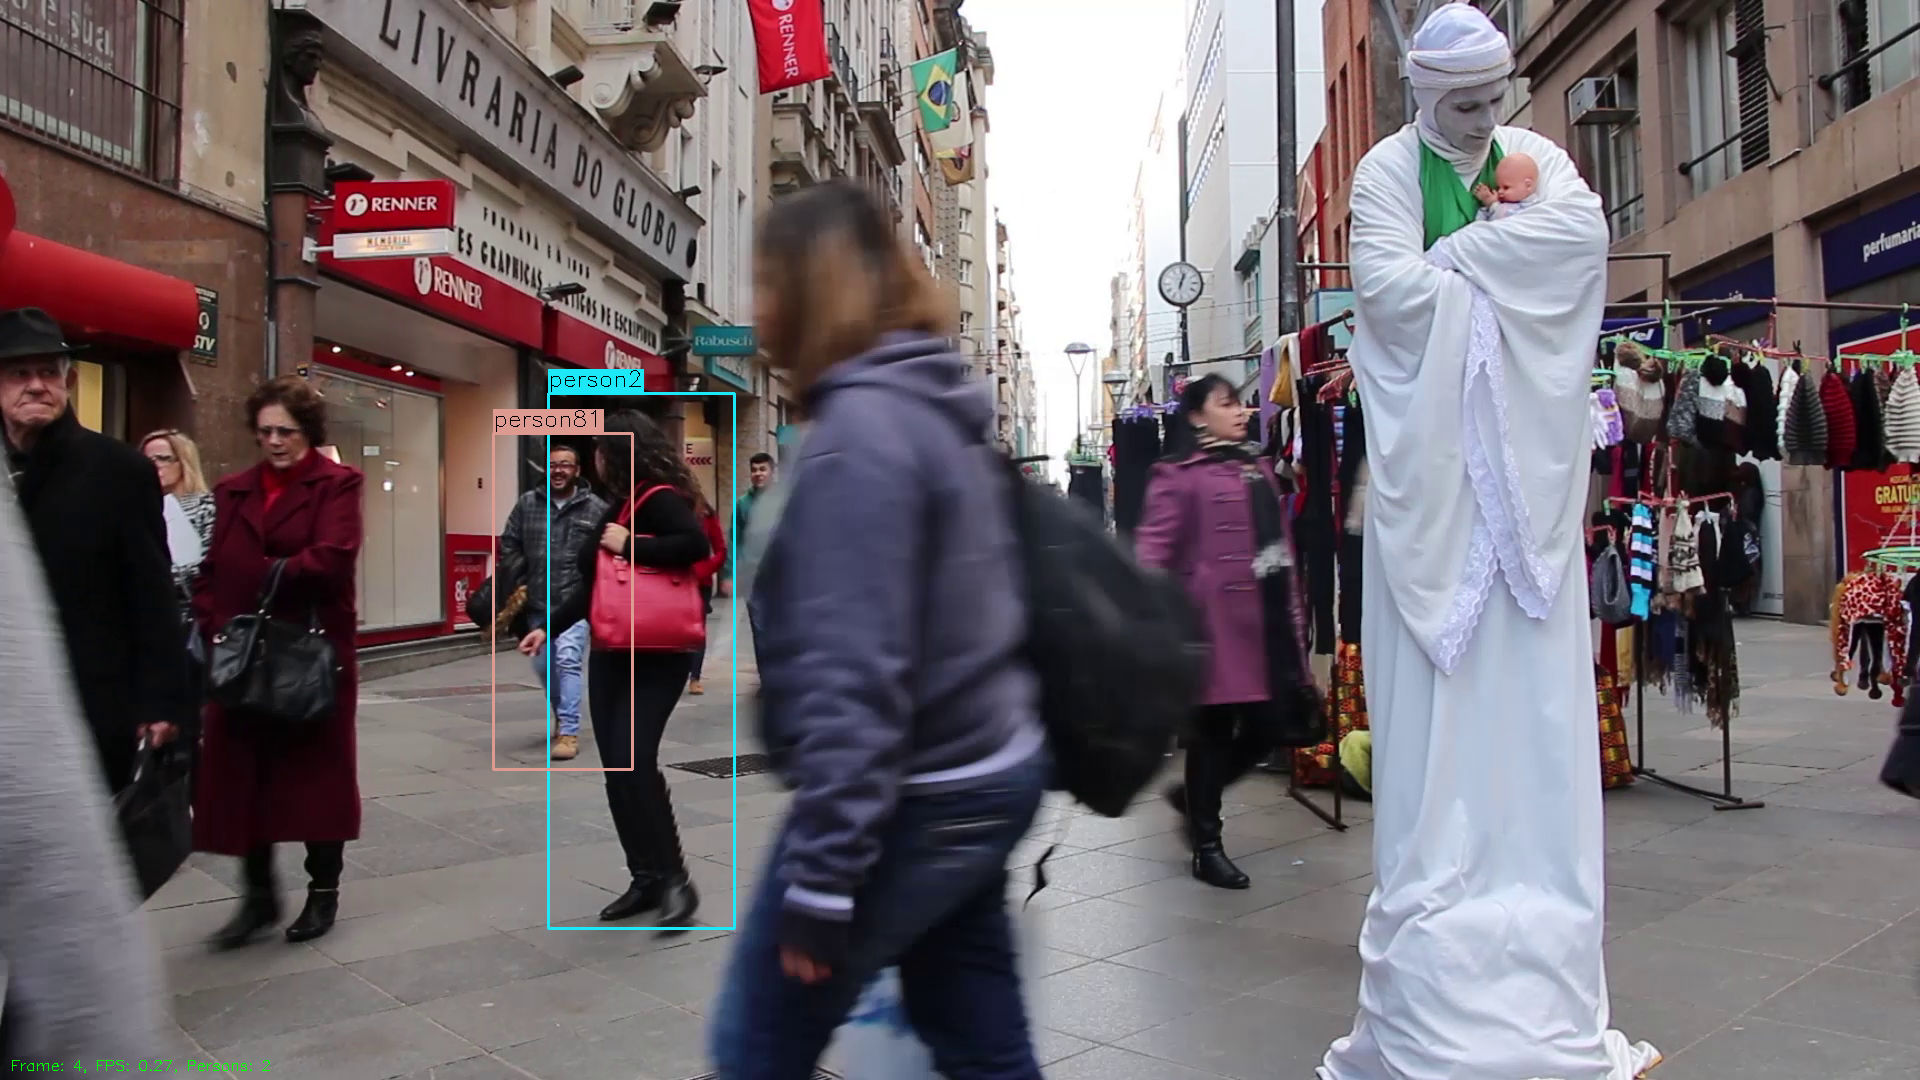
\includegraphics[width=\linewidth]{/home/luka/Workspaces/diplomski-rad/img/frame_4.png}
	\end{subfigure}
	\caption{Primjer detekcije Viola-Jones algoritmom}
	\label{img:violaJones-detection}
\end{figure}

\begin{table}[h]
\centering
\begin{tabular}{|rcl|}
\hline
	Broj vidljivih osoba po slici & & 5.67\\
\hline
	Broj detekcija po slici videa & & 4.91\\
\hline
	True Positivea po slici & & 3.59\\
\hline
	False Positivea po slici & & 1.32\\
\hline
	Preciznost (precision) & & 73.11\%\\
\hline
\end{tabular}
\caption{Rezultati Viola-Jones algoritma na videu Esquina Democratica}
\label{tab:viola-jones-result}
\end{table}

Viola-Jones algoritam vrlo je pouzdan i dolazi sa većinom biblioteka specijaliziranih za računalni vid (\textit{OpenCV}). Za razliku od YOLO-a, ovaj algoritam ima nešto više false-positivea. Nekoliko slika sa pogrešnim označavanjem prikazano je na slici \ref{img:violaJones-fp}. Još jedan od nedostataka ovog algoritma jest osjetljivost na različite fotometrijske značajke (promjene svijetlosti). 

\begin{figure}[htp]
	\centering
	\begin{subfigure}[b]{0.4\linewidth}
		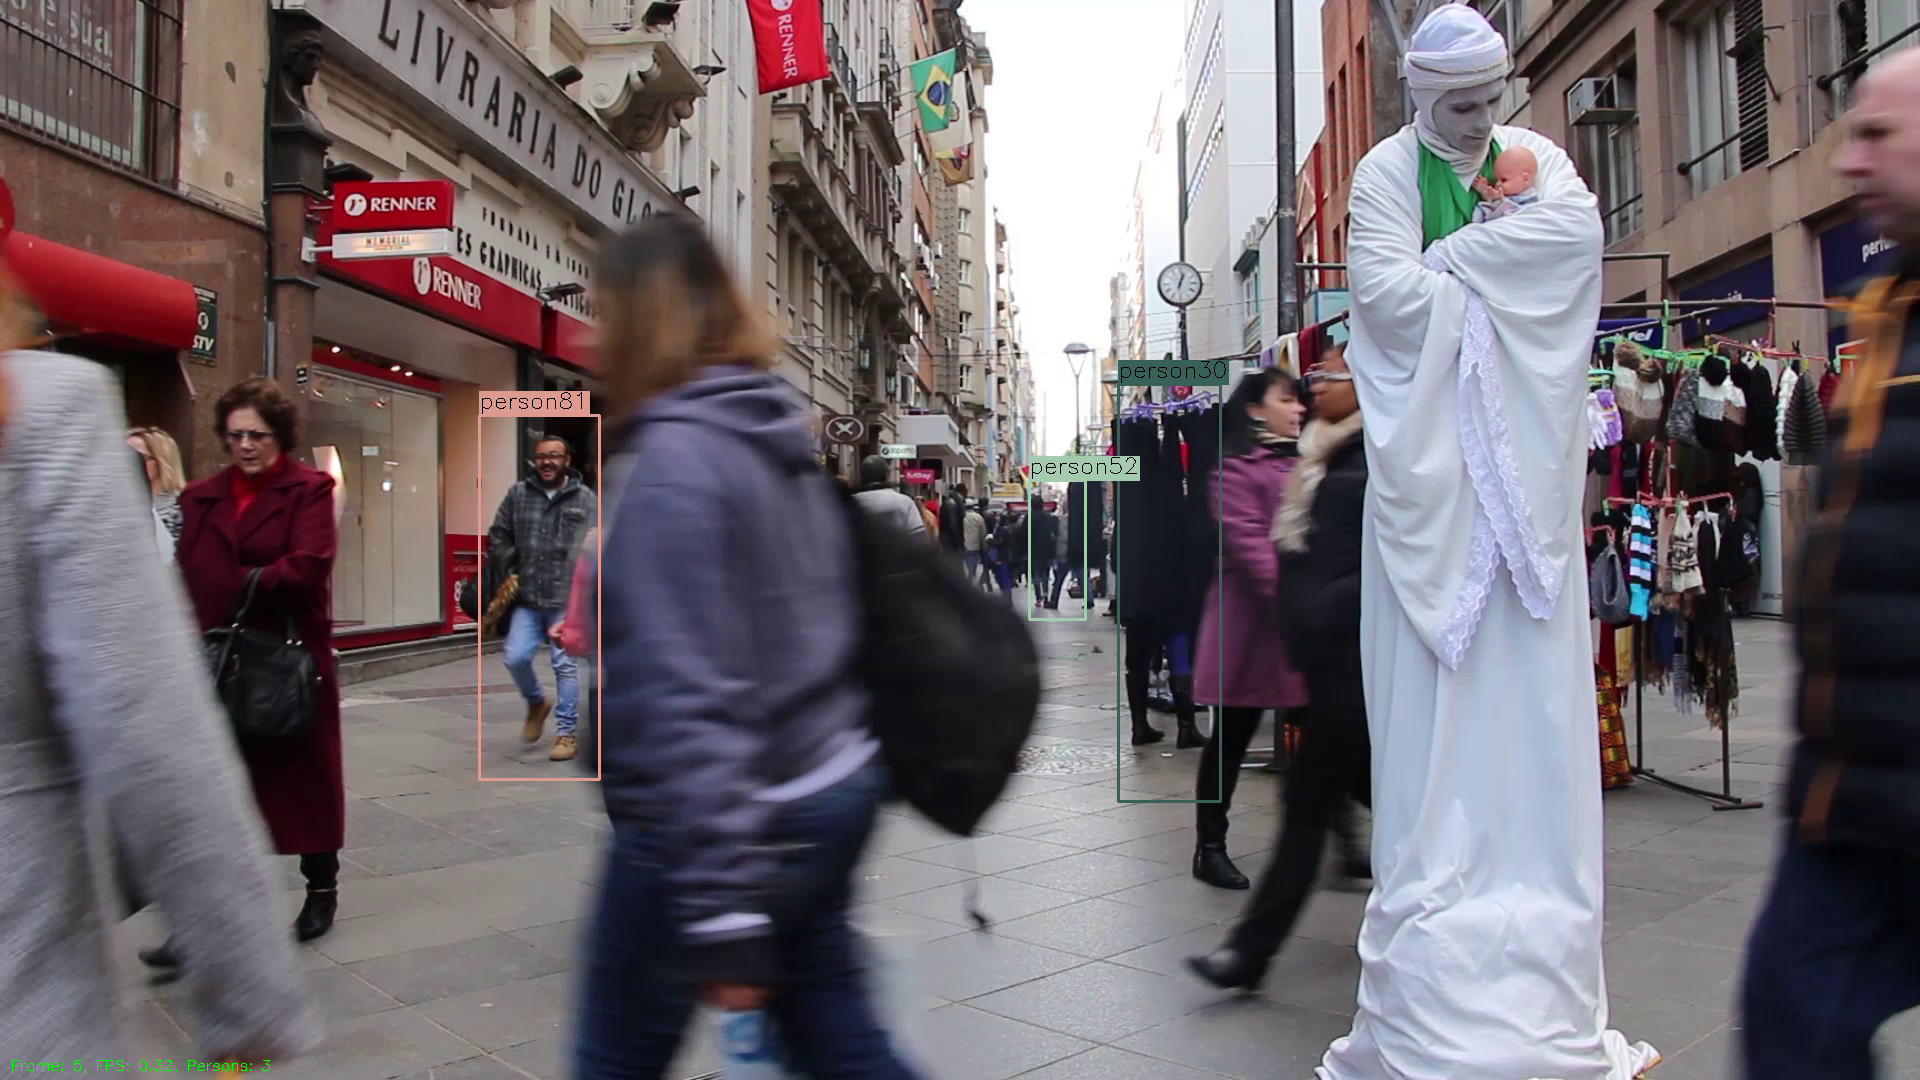
\includegraphics[width=\linewidth]{/home/luka/Workspaces/diplomski-rad/img/ViolaJonesFrames/frame_5.png}
	\end{subfigure}
	\begin{subfigure}[b]{0.4\linewidth}
		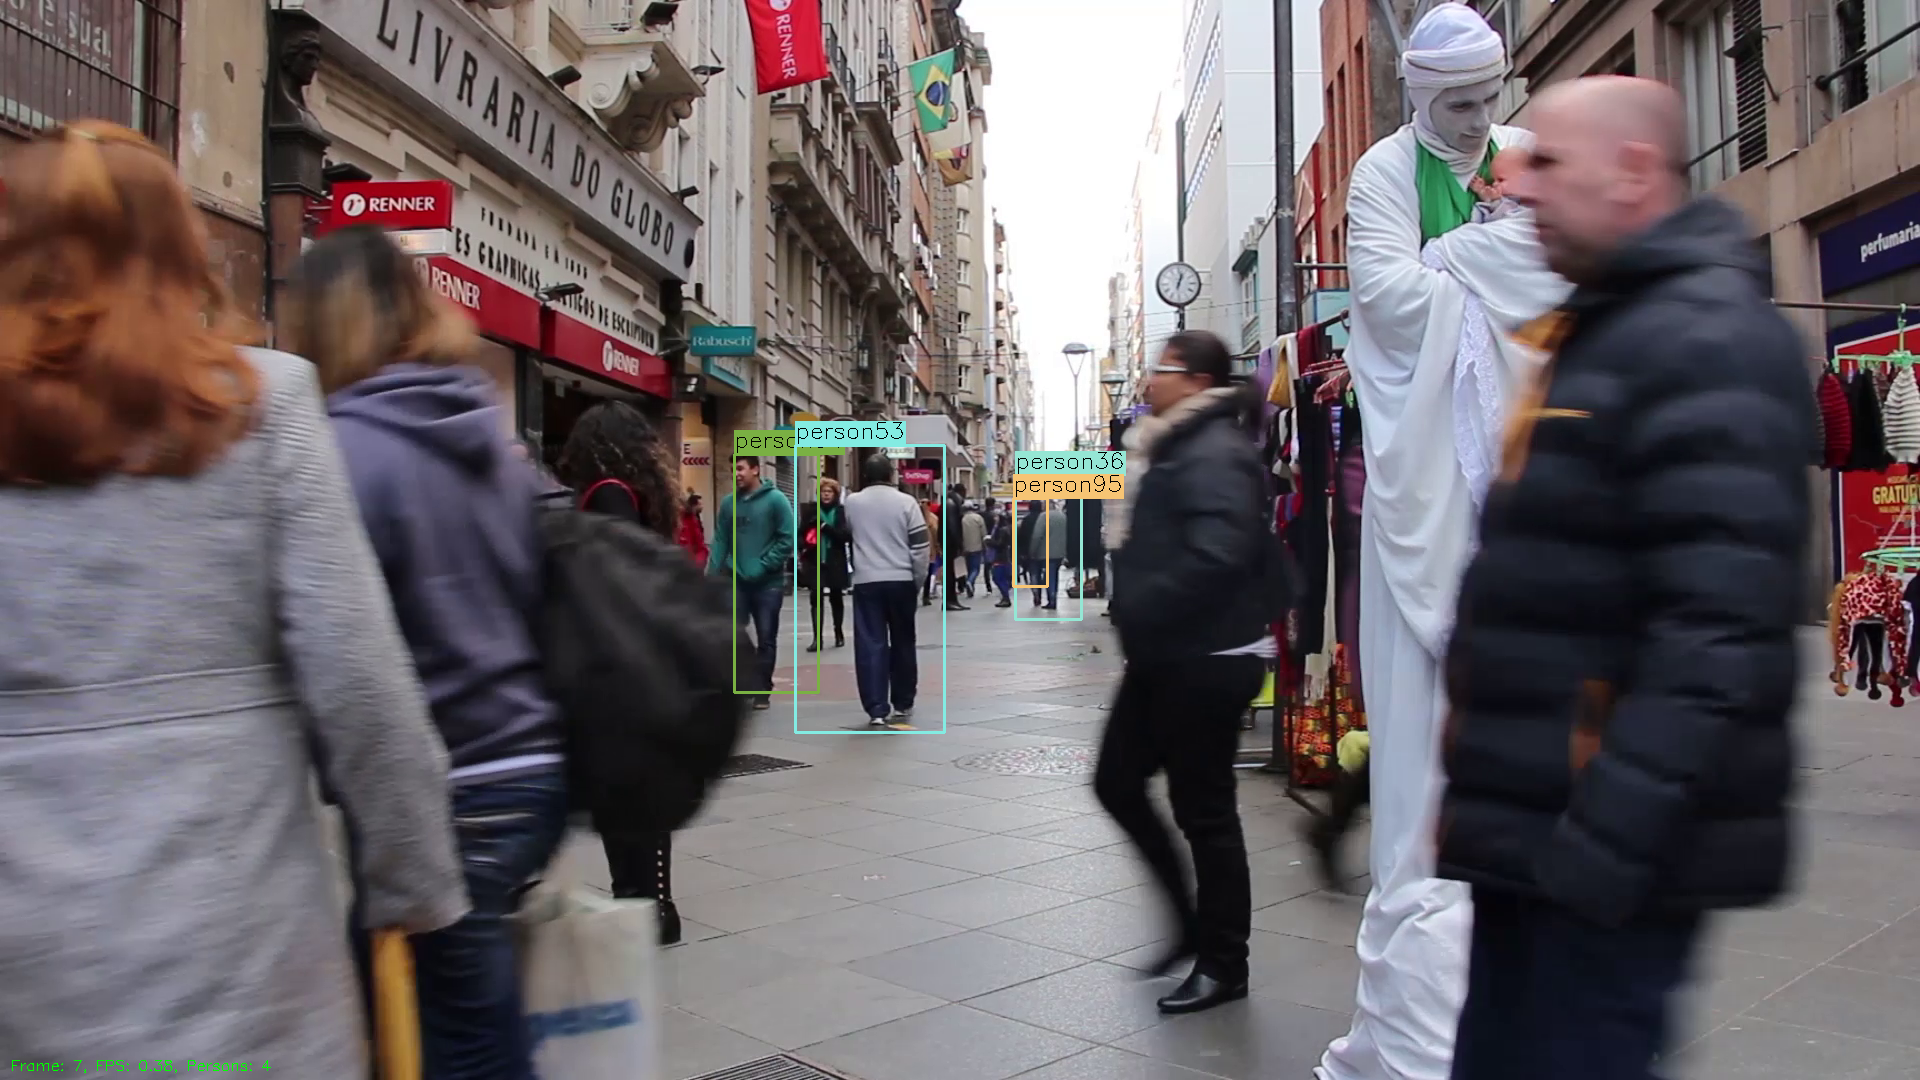
\includegraphics[width=\linewidth]{/home/luka/Workspaces/diplomski-rad/img/ViolaJonesFrames/frame_7.png}
	\end{subfigure}
	\begin{subfigure}[b]{0.4\linewidth}
		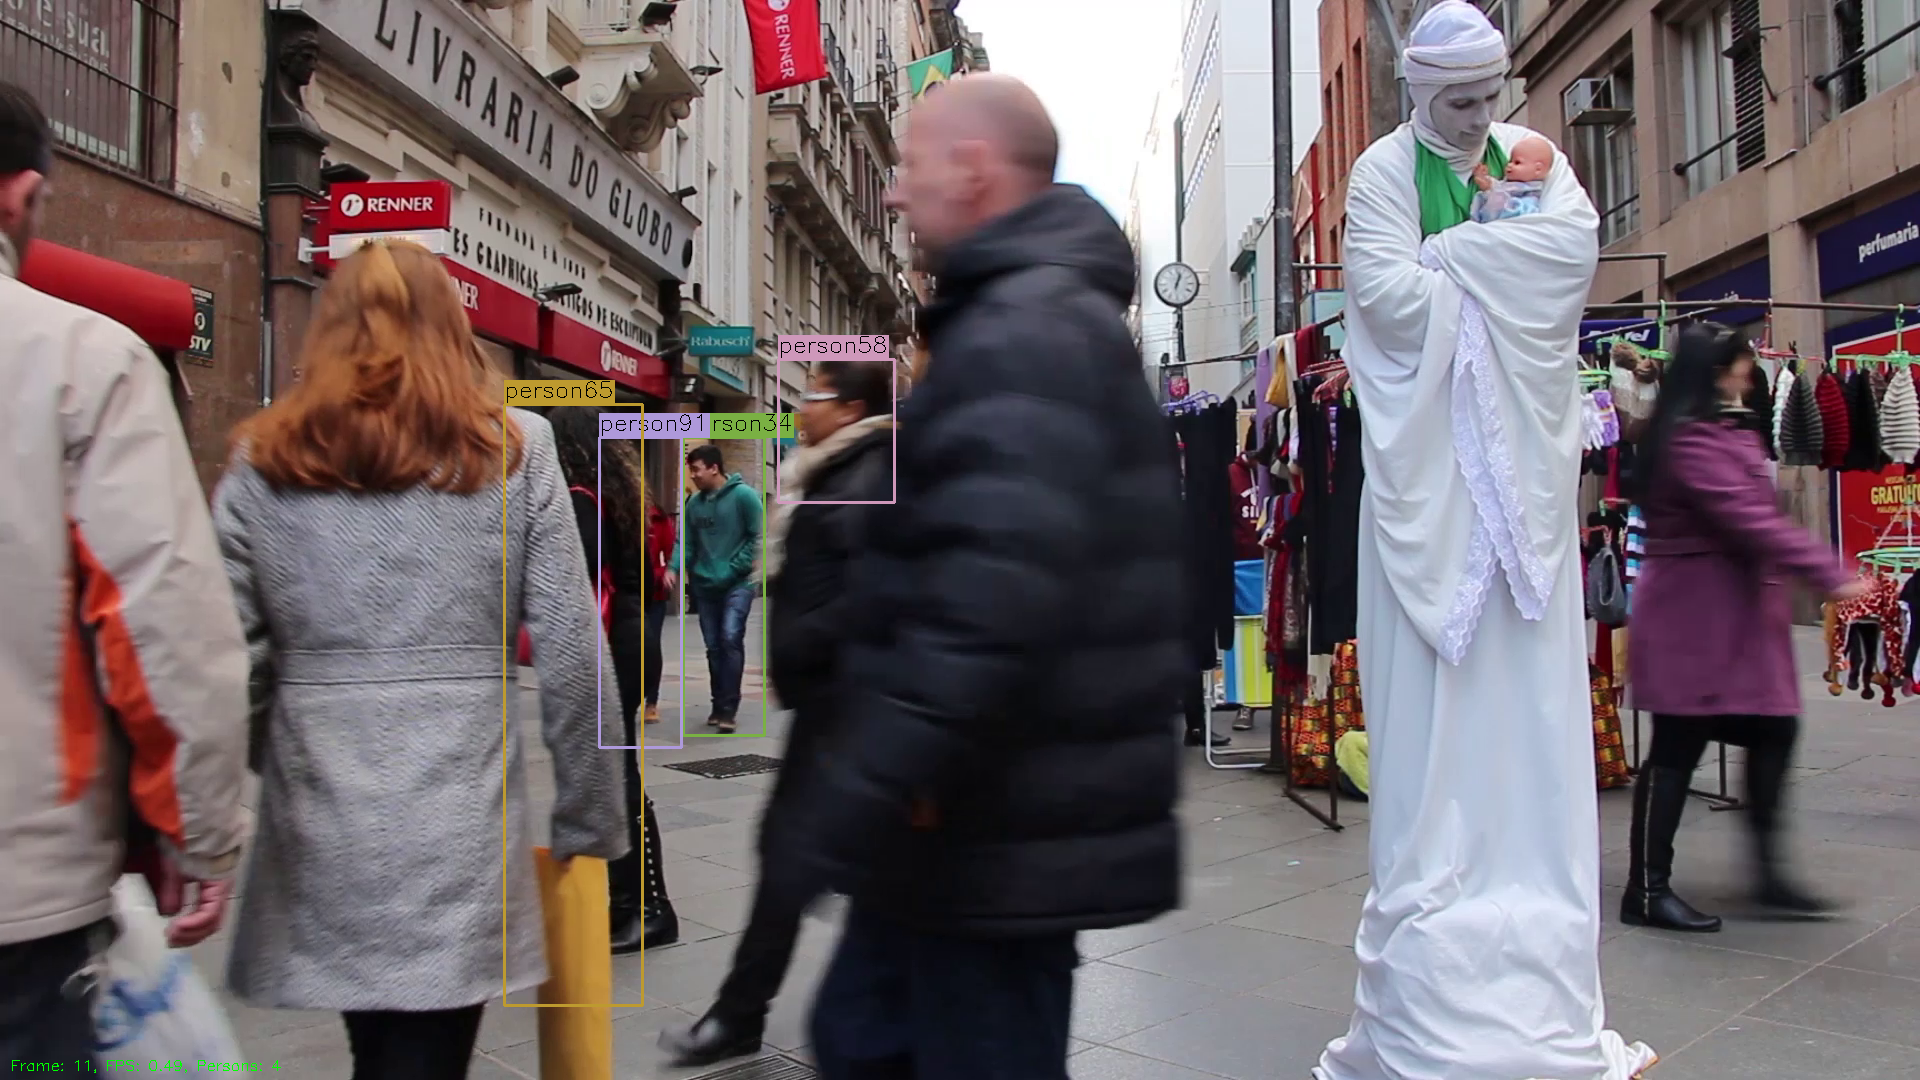
\includegraphics[width=\linewidth]{/home/luka/Workspaces/diplomski-rad/img/ViolaJonesFrames/frame_11.png}
	\end{subfigure}
	\begin{subfigure}[b]{0.4\linewidth}
		\includegraphics[width=\linewidth]{/home/luka/Workspaces/diplomski-rad/img/ViolaJonesFrames/frame_17.png}
	\end{subfigure}
	\caption{Primjer false positive detekcije Viola-Jones algoritma}
	\label{img:violaJones-fp}
\end{figure}

\section{YOLO}

Ovaj je algoritam, u originalnom obliku, implementiran u programskom jeziku C te je izuzetno brz. U radu se spominje da na grafičkoj kartici NVidia Titan X postiže brzine od 45 do 90 FPS (\textit{engl. Frames Per Second}) što je izuzetno brzo, uzimajući u obzir i izvanrednu točnost modela. Implementacija u ovom radu je nešto sporija zbog nekoliko razloga: agloritam je implementiran u programskom jeziku Python, a što je još važnije, izvršava se na procesoru (CPU).

U ovoj implementaciji za procesiranje slike potrebno je vrijeme od 3.5 do 6 sekundi, ovisno o slici. Tu je uračunato nekoliko komponenti čija se vremena izvođenja nalaze u tablici \ref{tab:img-performance} te slici \ref{img:img-performance-terminal}.

\begin{center}
\begin{lstlisting}[language=Awk, caption=Poziv programa za jednu sliku]
python3 eval.py image='path/to/image'
\end{lstlisting}
\end{center}

\begin{table}[h]
\centering
\begin{tabular}{||c|c||}
\hline
\hline
	Obrada slike & 3.9219 s\\
\hline
	Stvaranje modela & 2.717 s\\
\hline
	Predviđanje sa slike & 1.201 s\\
\hline
	Postprocesiranje & 0.0003 s\\
\hline
	Iscrtavanje okvira & 0.0002 s\\
\hline
\hline
\end{tabular}
\caption{Vrijeme izvođenja pojedinih dijelova programa za obradu slike}
\label{tab:img-performance}
\end{table}

\begin{figure}[htp]
	\centering
	\begin{subfigure}[b]{0.7\linewidth}
		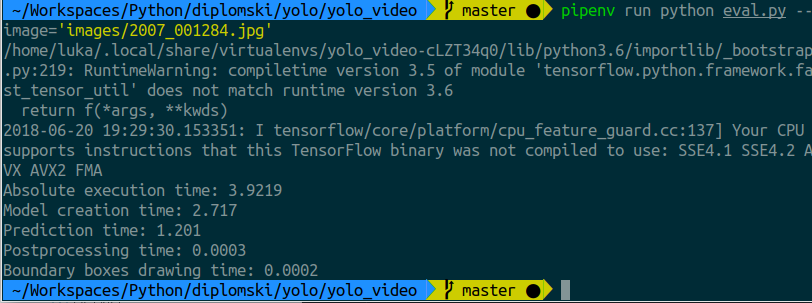
\includegraphics[width=\linewidth]{/home/luka/Workspaces/diplomski-rad/img/evaluation_timer.png}
		\caption{Vrijeme izvođenja pojedinih dijelova programa za obradu slike}
		\label{img:img-performance-terminal}
	\end{subfigure}
	\begin{subfigure}[b]{0.7\linewidth}
		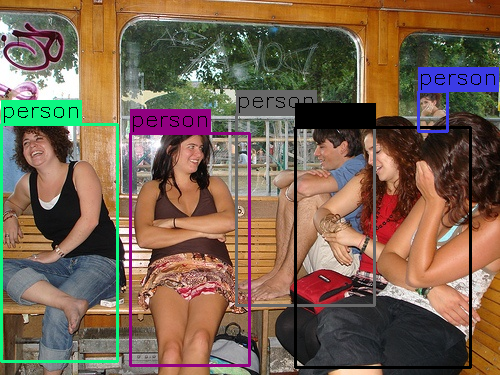
\includegraphics[width=\linewidth]{/home/luka/Workspaces/diplomski-rad/img/eval-img.png}
		\caption{Slika sa označenim detektiranim objektima}
		\label{img:img-result}
	\end{subfigure}
	\caption{Rezultat pokretanja algoritma na slici}
	\label{img:img-performance}
\end{figure}

Danas je detekcija objekata na slikama vrlo dobro riješena. Kao što je bilo govora na početku poglavlja o detekciji konvolucijskim mrežama, problem slike odlično riješavaju modeli koji imaju klasifikaciju i lokalizaciju odvojenu, koji izrezuju dijelove slike i ponovo ih dovode na ulaze mreža. Primjer jednog takvog algoritma je i \textit{Tiny Face Detector} opisan u istoimenom radu \citep{TinyFaceDetector}. No, ti algoritmi su izuzetno spori zbog gore navedenih razloga. Njima nije naglasak na performansama, nego isključivo na točnosti i preciznosti.

Ovaj algoritam je, kao predvodnik u kategoriji algoritama za detekciju objekata, zapravo dizajniran za brzo izvođenje i primjenu na videu, uz minimalne gubitke točnosti i preciznosti. 

\begin{figure}[htp]
	\centering
	\begin{subfigure}[b]{0.4\linewidth}
		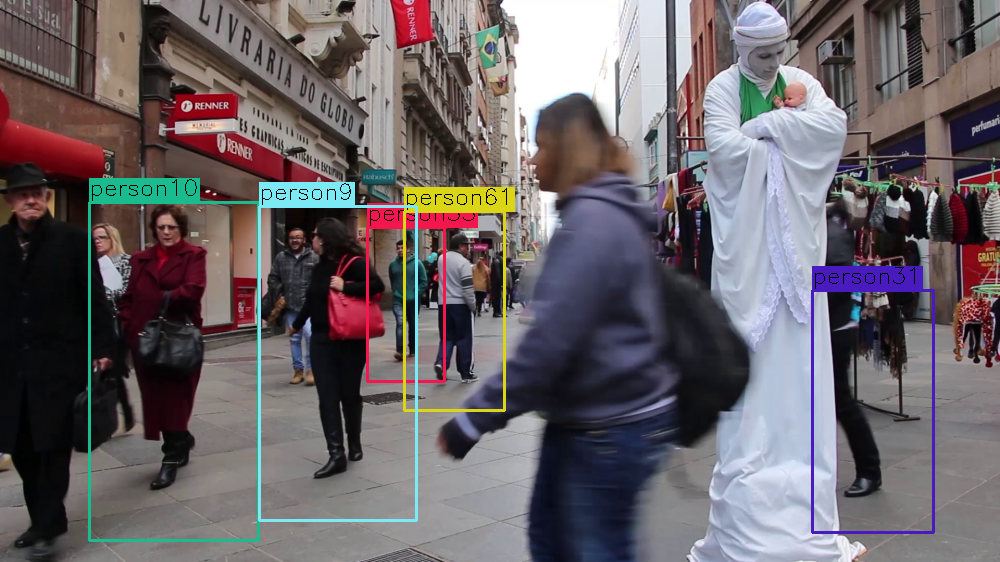
\includegraphics[width=\linewidth]{/home/luka/Workspaces/diplomski-rad/img/frame_16.png}
	\end{subfigure}
	\begin{subfigure}[b]{0.4\linewidth}
		\includegraphics[width=\linewidth]{/home/luka/Workspaces/diplomski-rad/img/frame_17.png}
	\end{subfigure}
	\begin{subfigure}[b]{0.4\linewidth}
		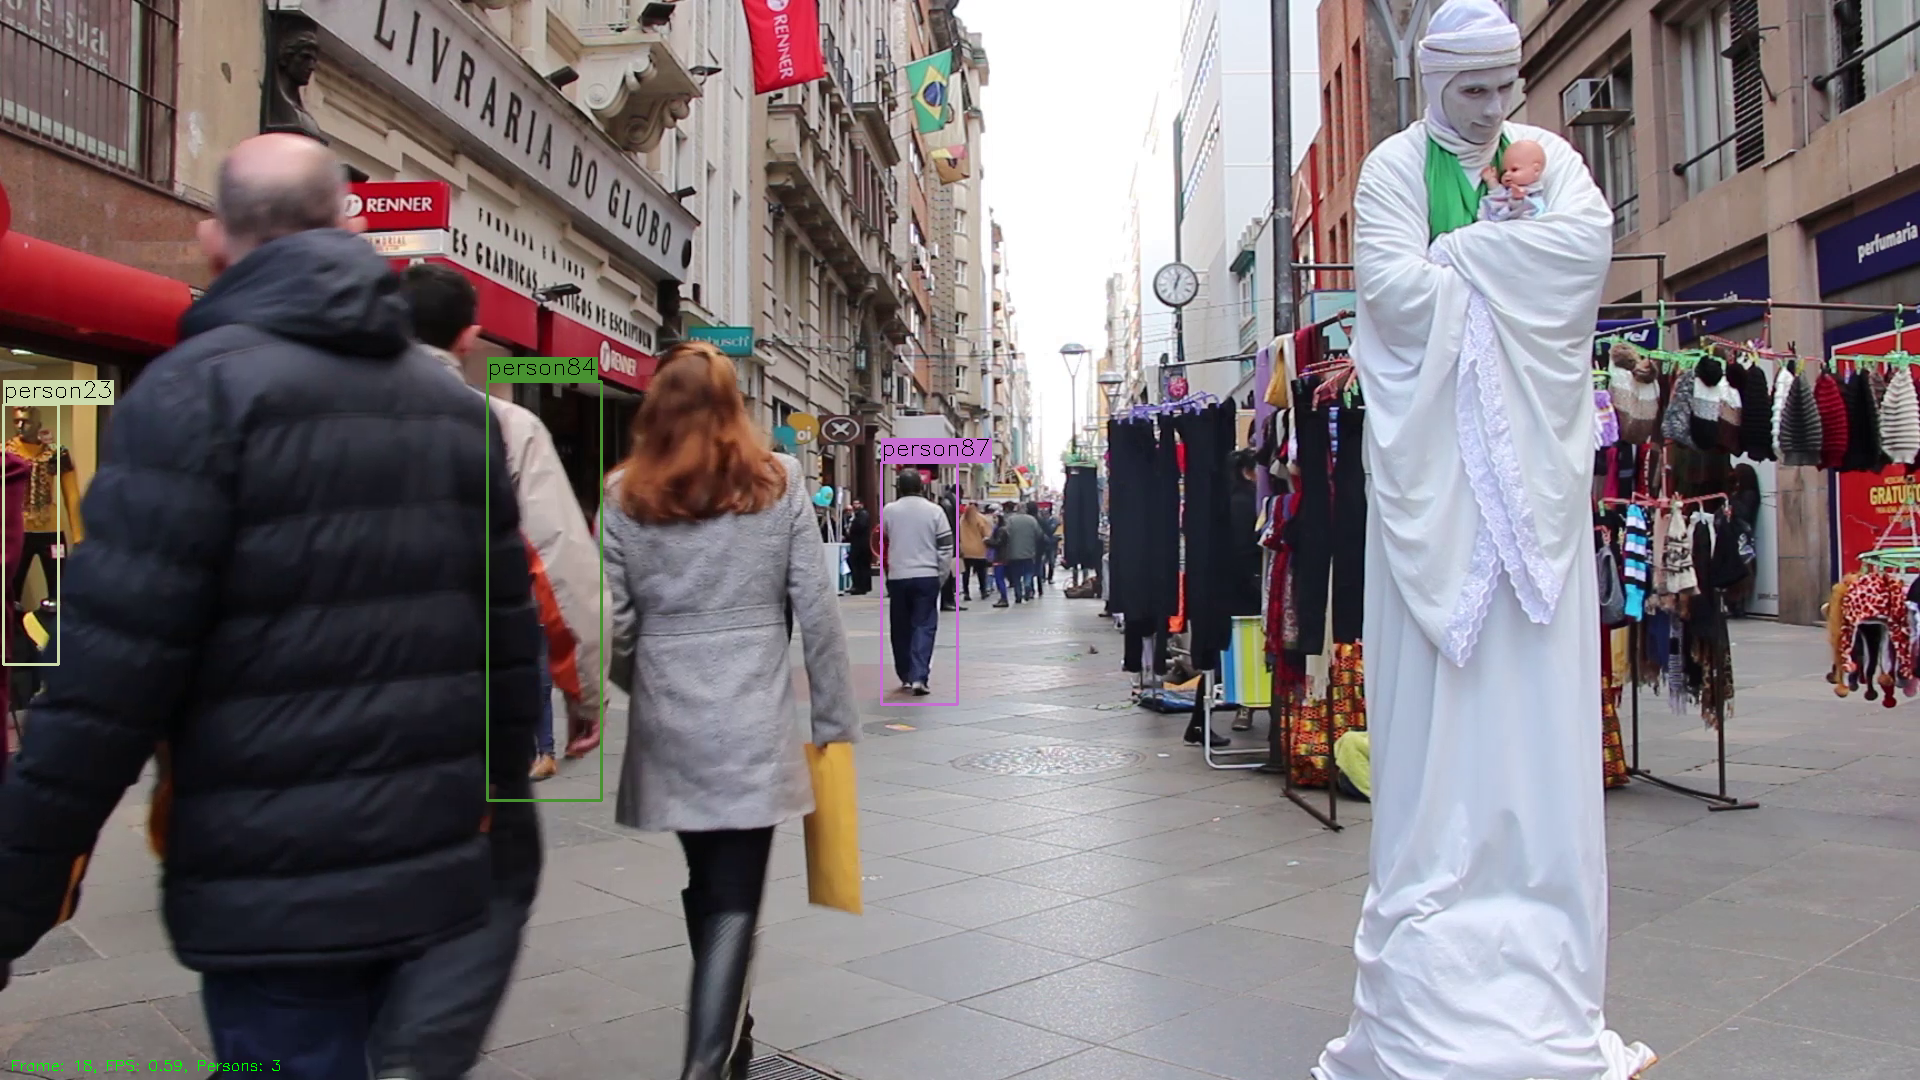
\includegraphics[width=\linewidth]{/home/luka/Workspaces/diplomski-rad/img/frame_18.png}
	\end{subfigure}
	\begin{subfigure}[b]{0.4\linewidth}
		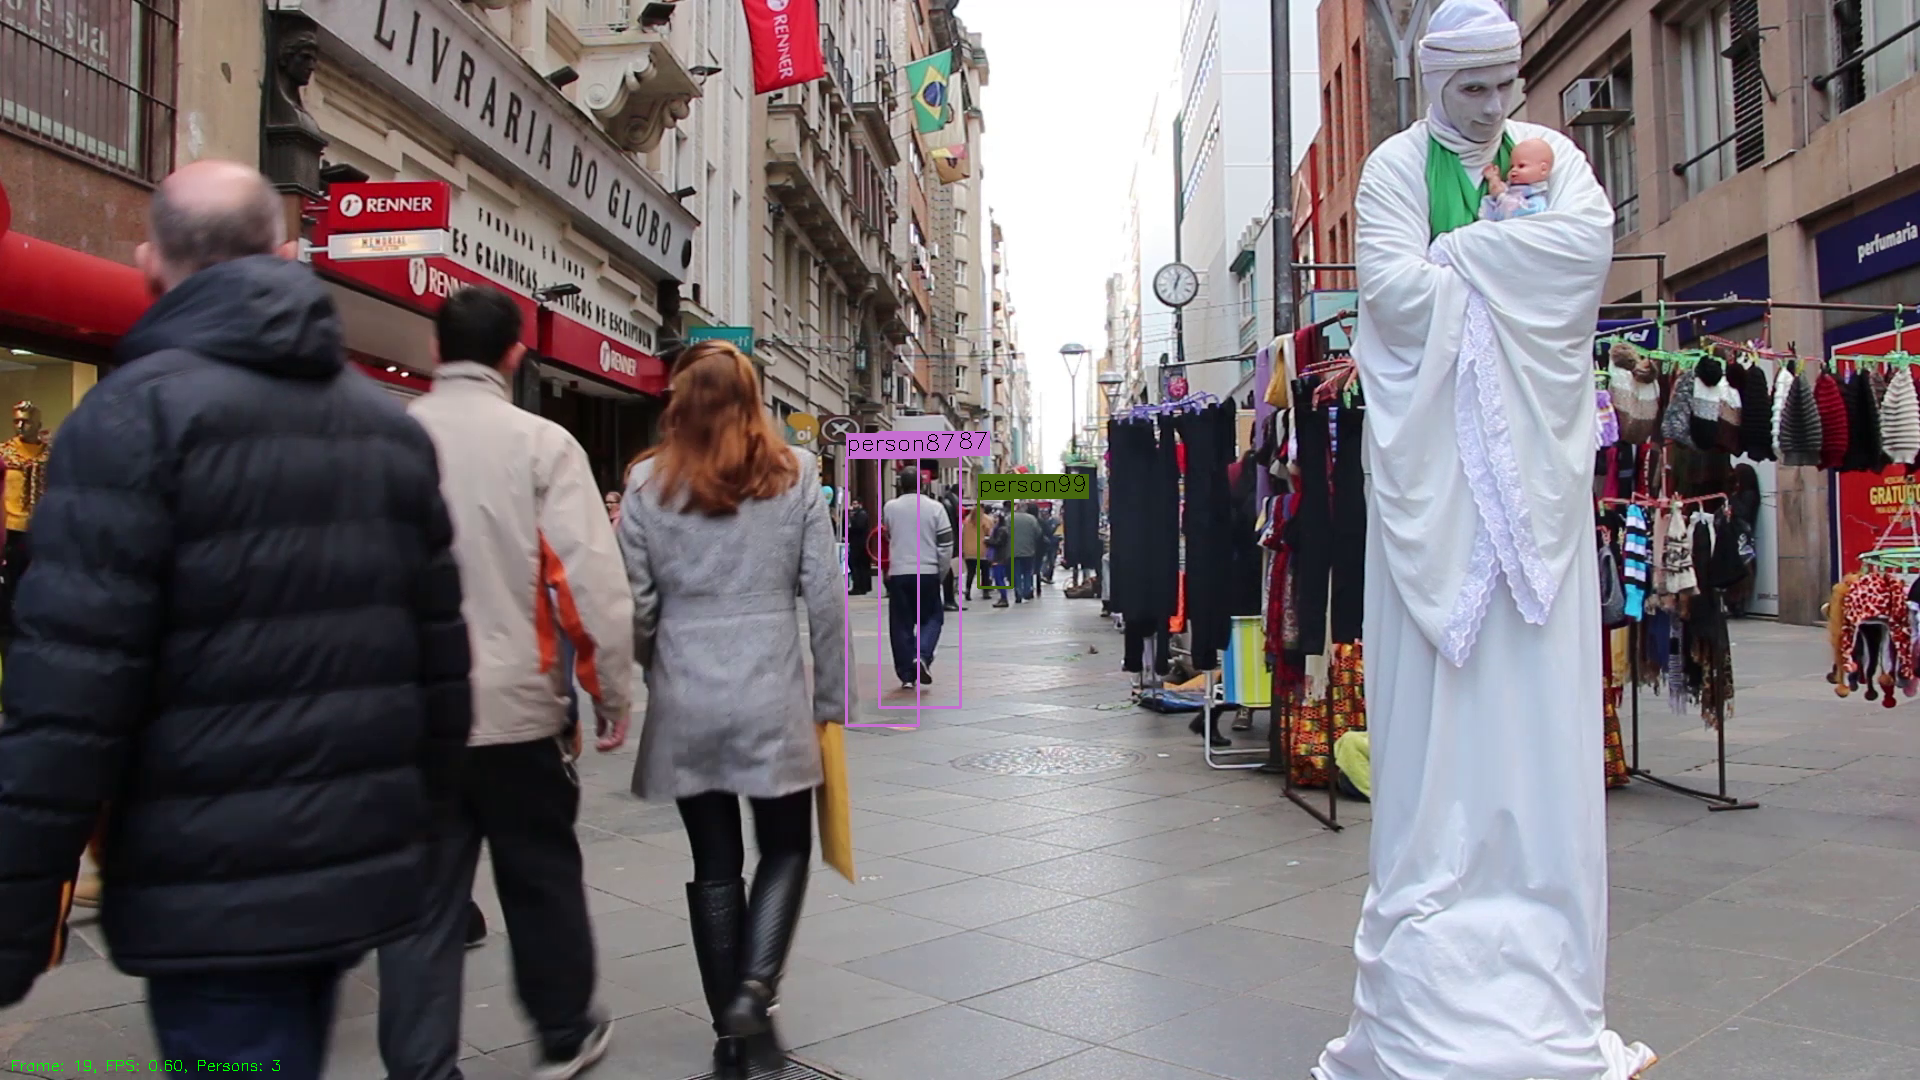
\includegraphics[width=\linewidth]{/home/luka/Workspaces/diplomski-rad/img/frame_19.png}
	\end{subfigure}
	\begin{subfigure}[b]{0.4\linewidth}
		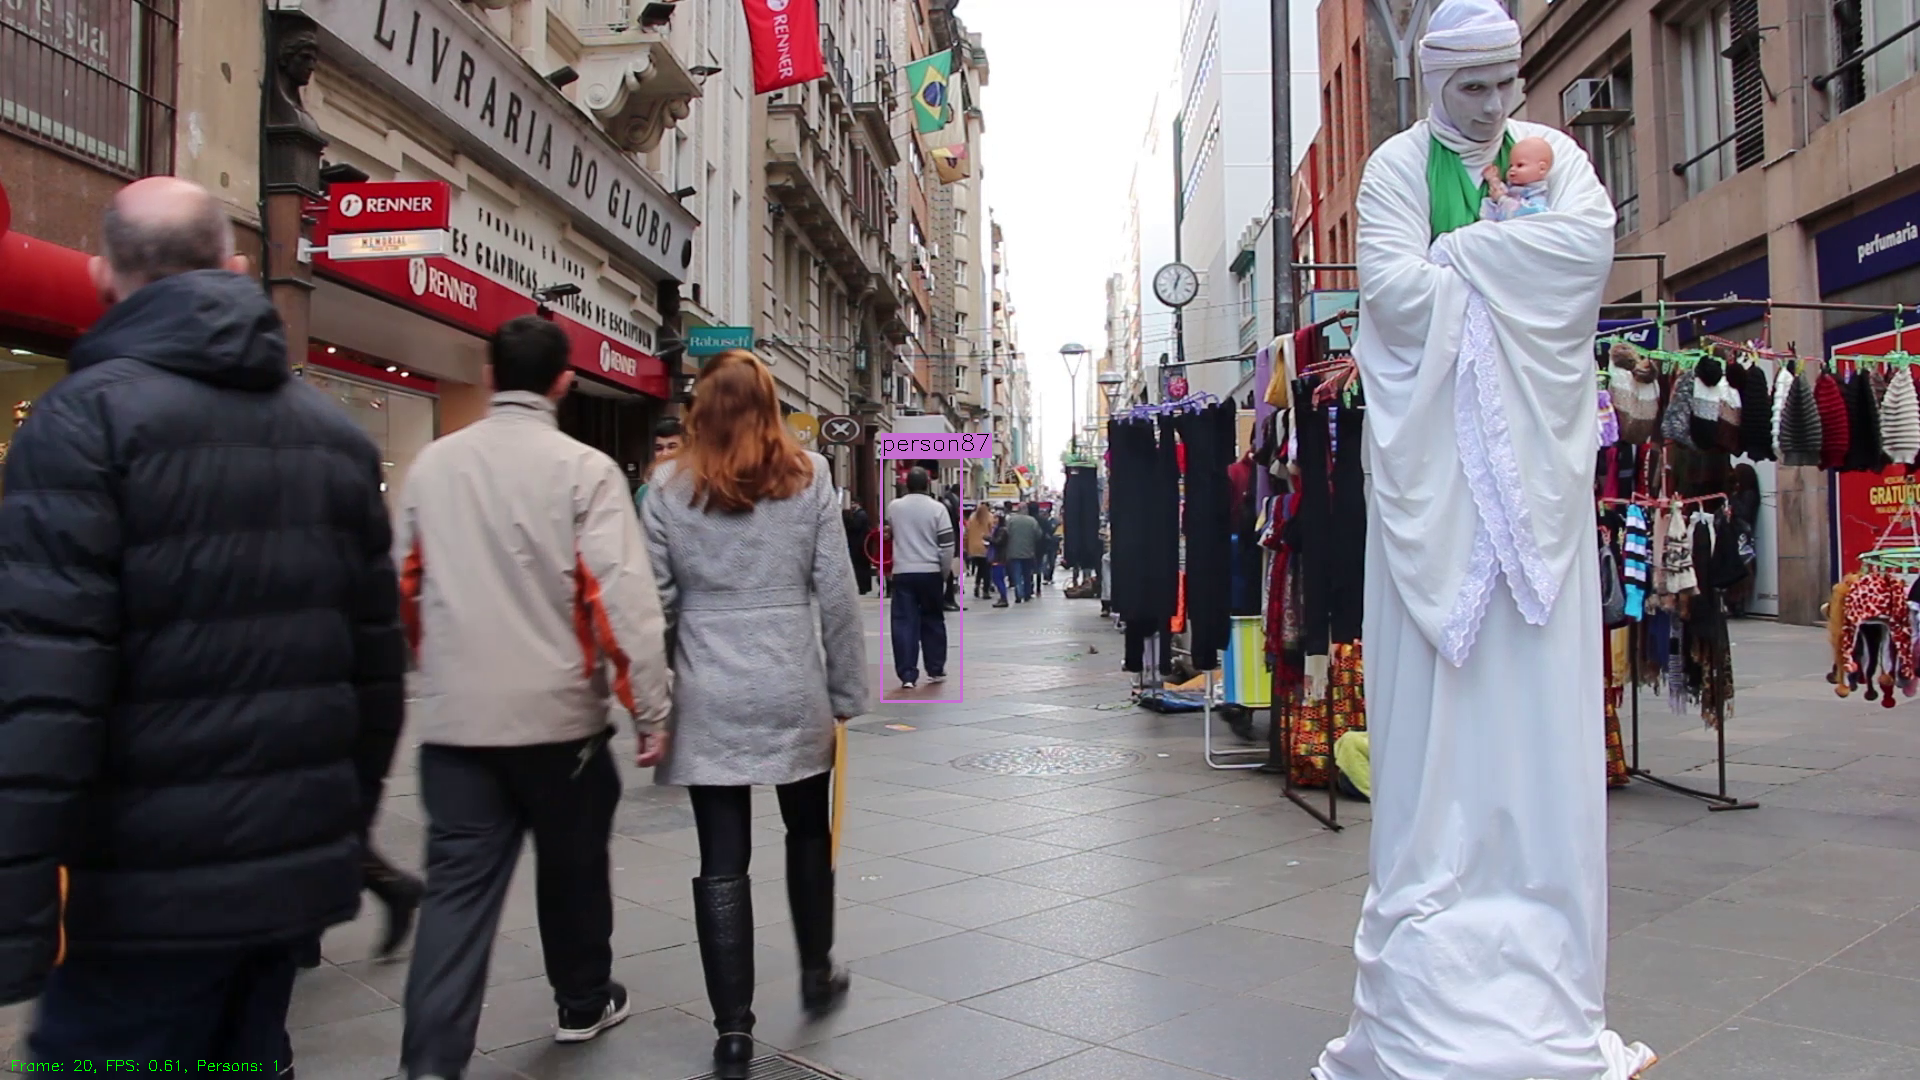
\includegraphics[width=\linewidth]{/home/luka/Workspaces/diplomski-rad/img/frame_20.png}
	\end{subfigure}
	\begin{subfigure}[b]{0.4\linewidth}
		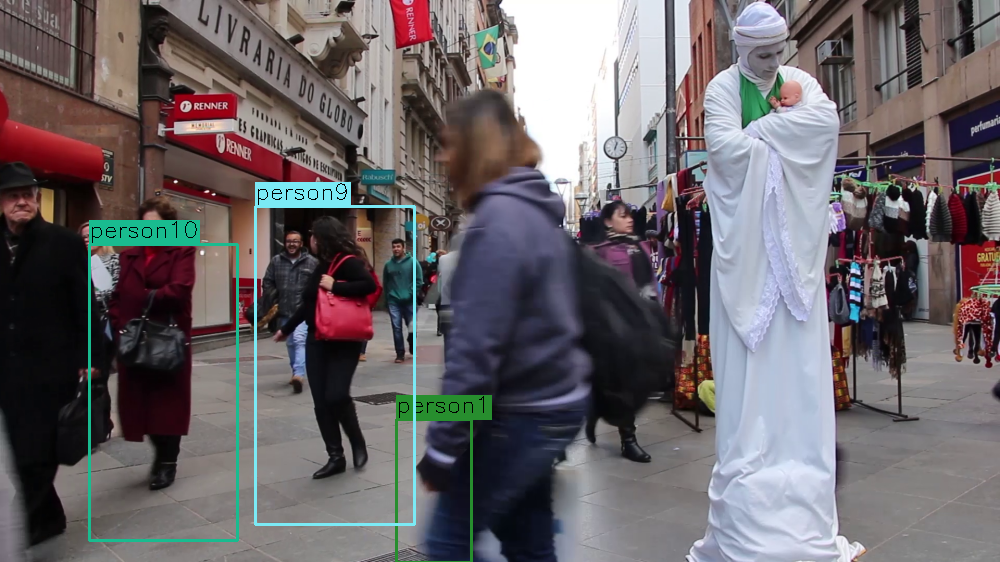
\includegraphics[width=\linewidth]{/home/luka/Workspaces/diplomski-rad/img/frame_21.png}
	\end{subfigure}
	\begin{subfigure}[b]{0.4\linewidth}
		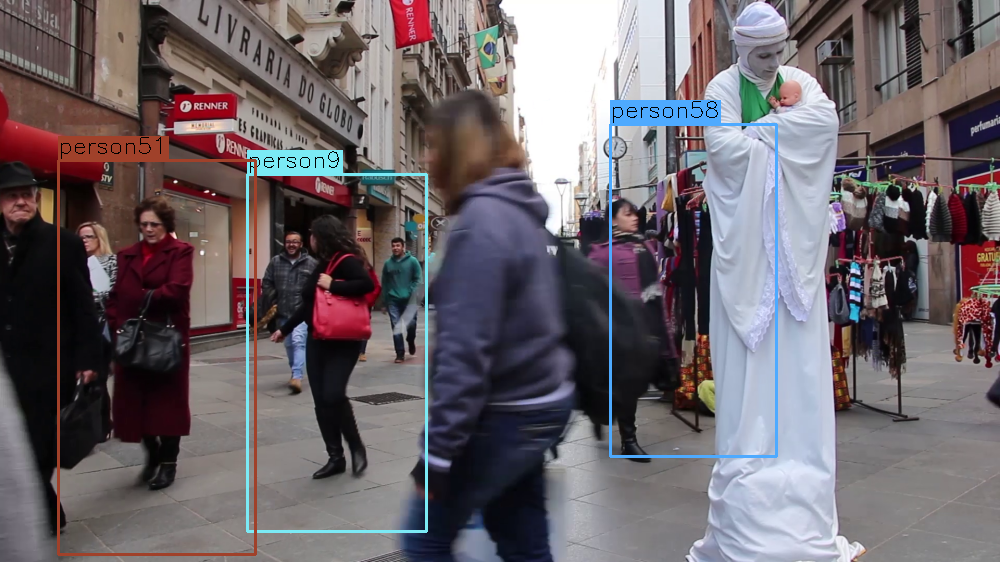
\includegraphics[width=\linewidth]{/home/luka/Workspaces/diplomski-rad/img/frame_22.png}
	\end{subfigure}
	\begin{subfigure}[b]{0.4\linewidth}
		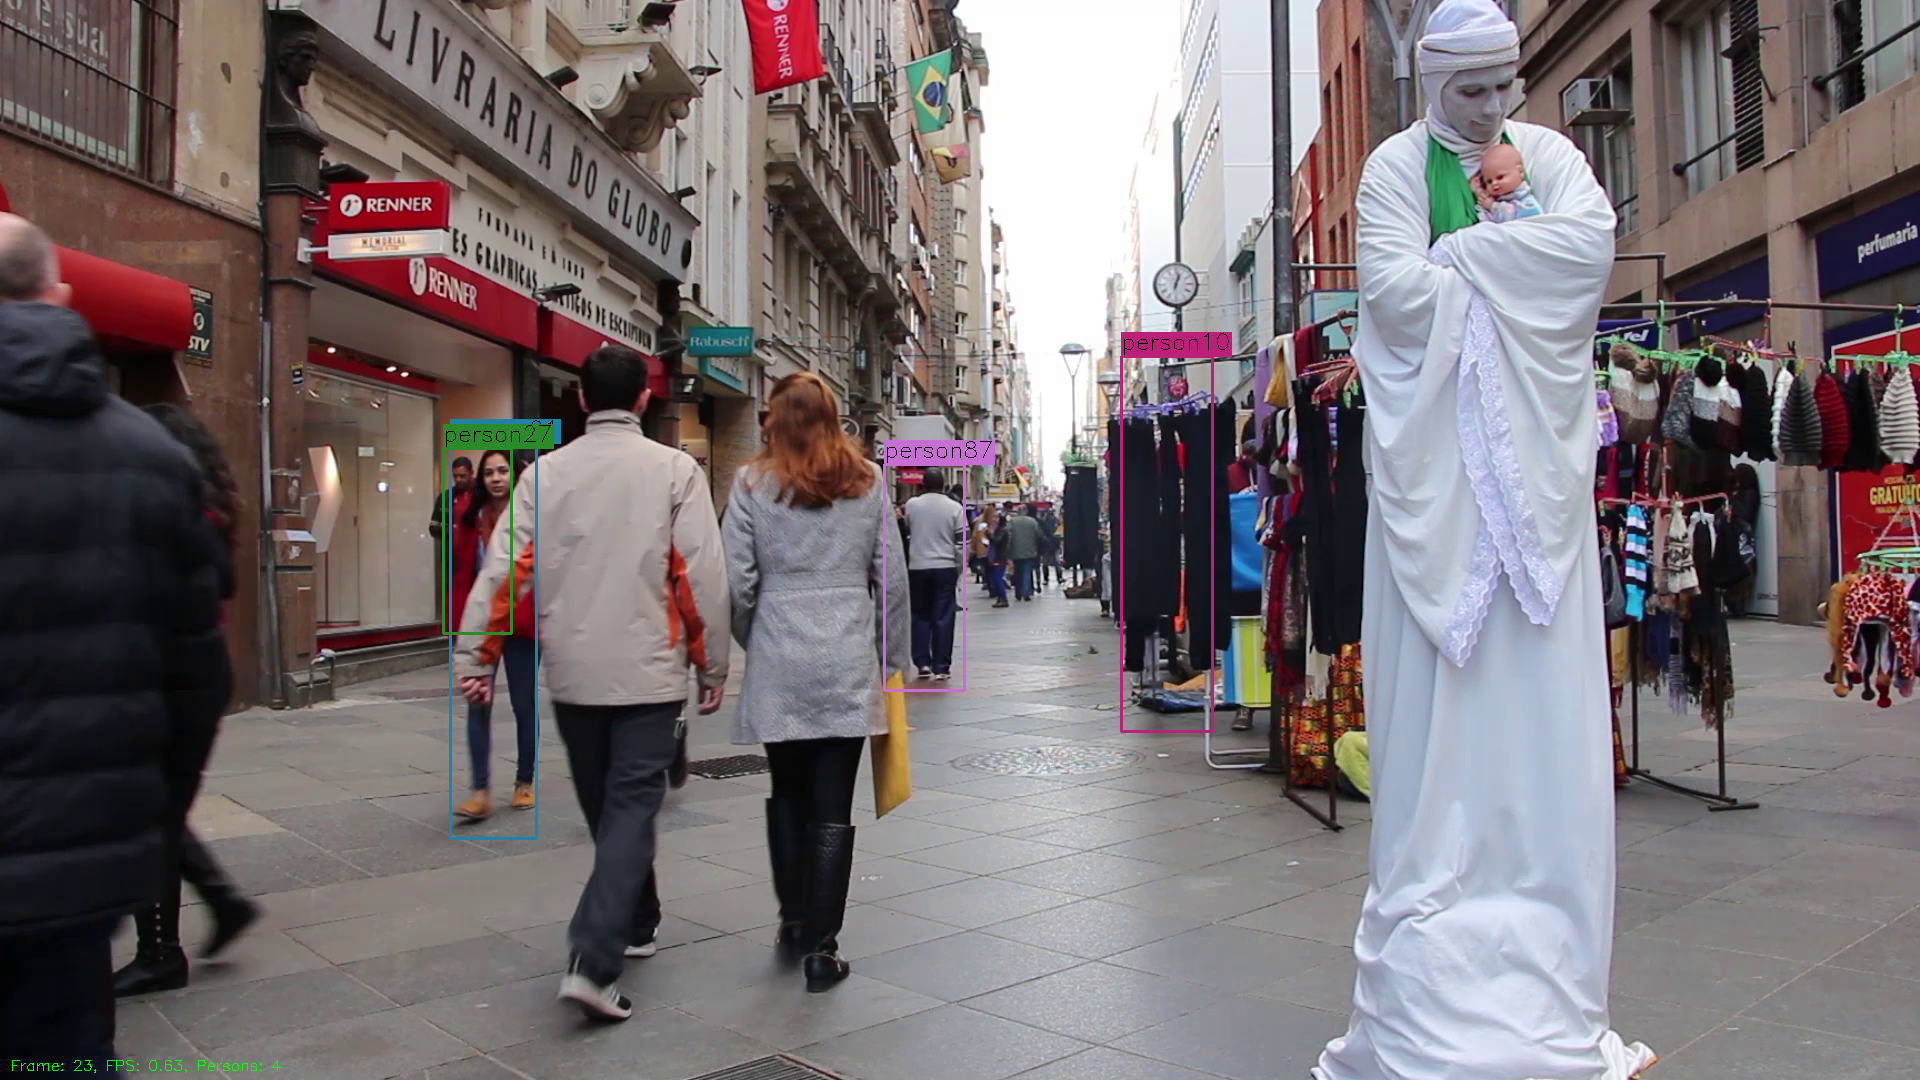
\includegraphics[width=\linewidth]{/home/luka/Workspaces/diplomski-rad/img/frame_23.png}
	\end{subfigure}
	\begin{subfigure}[b]{0.4\linewidth}
		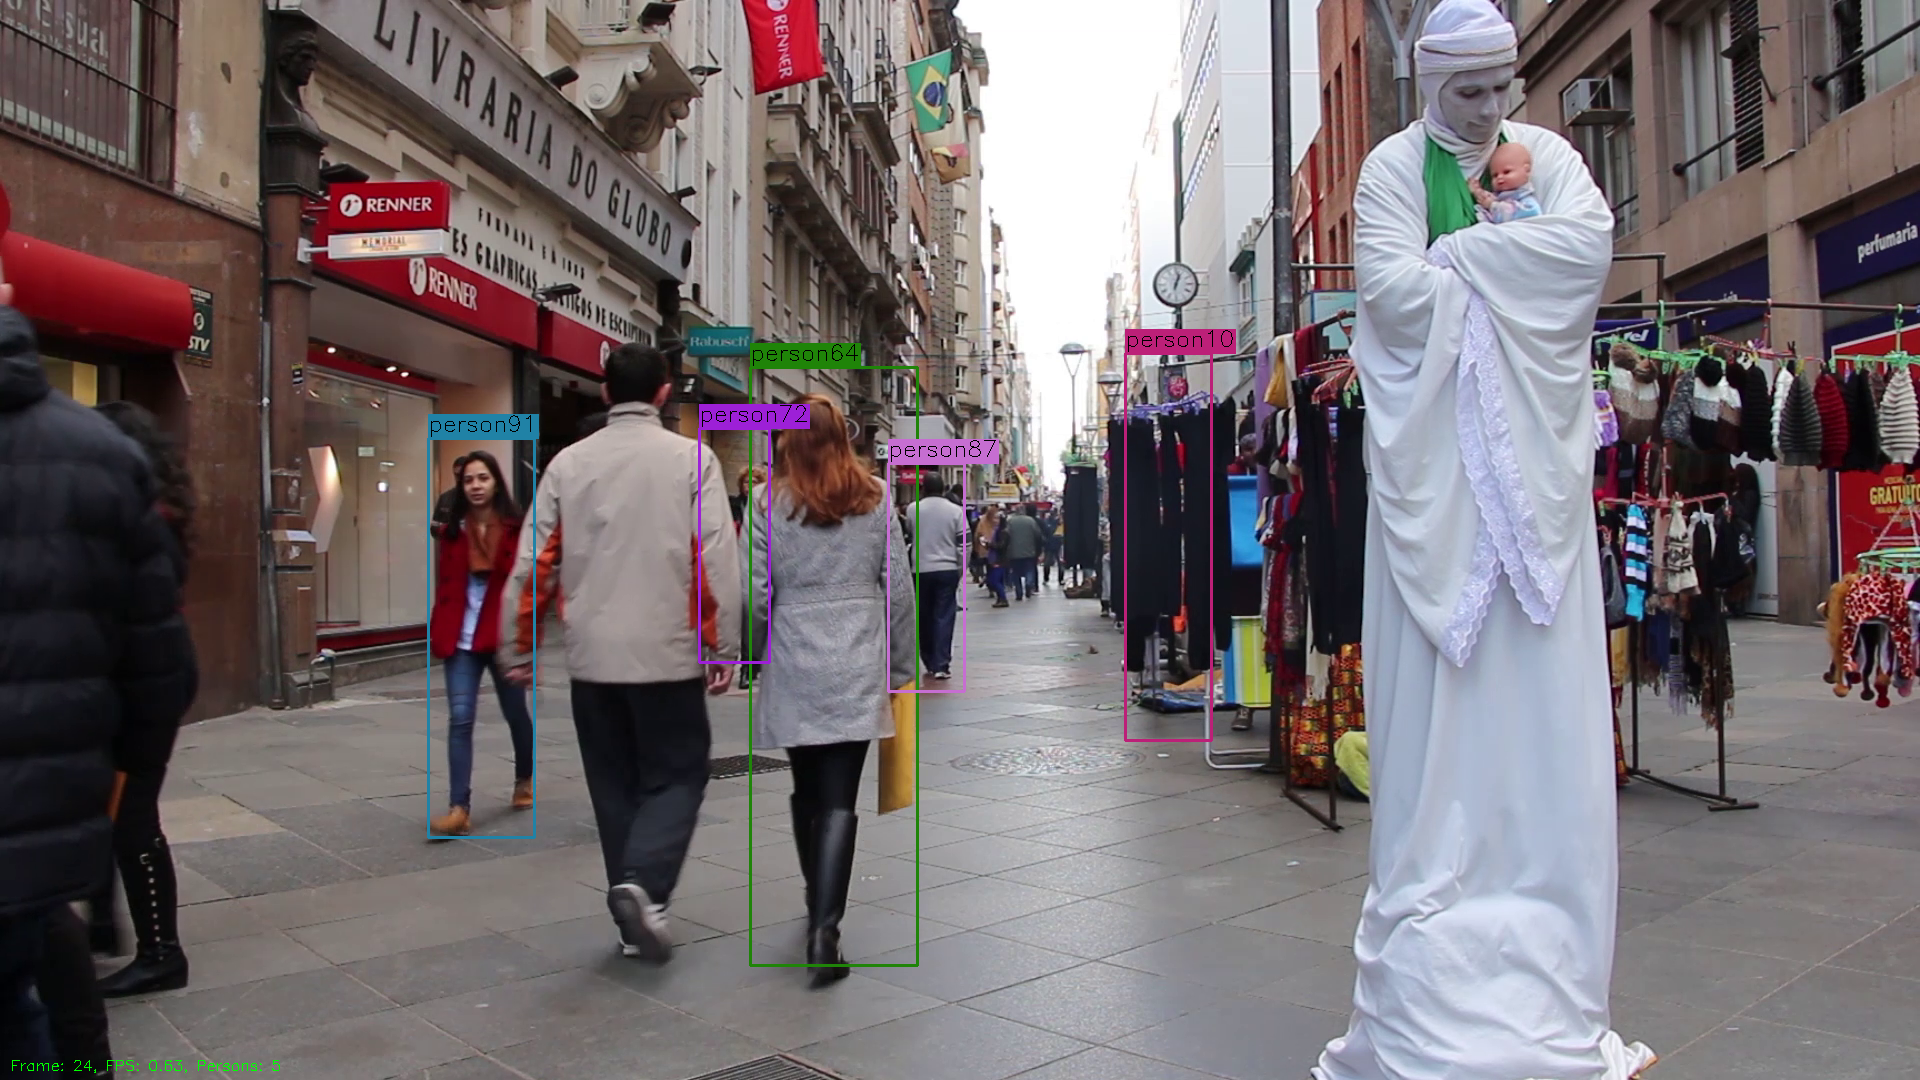
\includegraphics[width=\linewidth]{/home/luka/Workspaces/diplomski-rad/img/frame_24.png}
	\end{subfigure}
	\begin{subfigure}[b]{0.4\linewidth}
		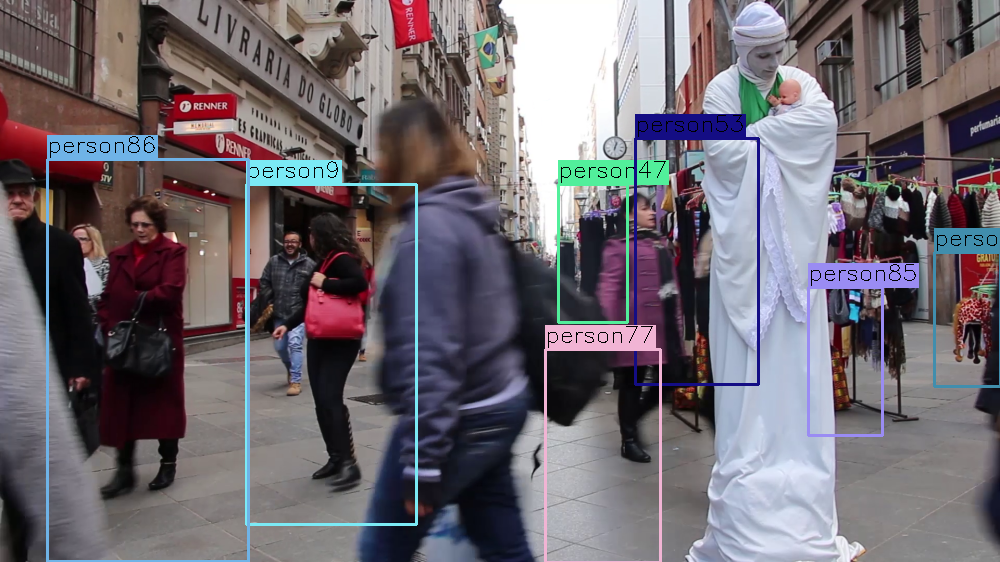
\includegraphics[width=\linewidth]{/home/luka/Workspaces/diplomski-rad/img/frame_25.png}
	\end{subfigure}
	\begin{subfigure}[b]{0.4\linewidth}
		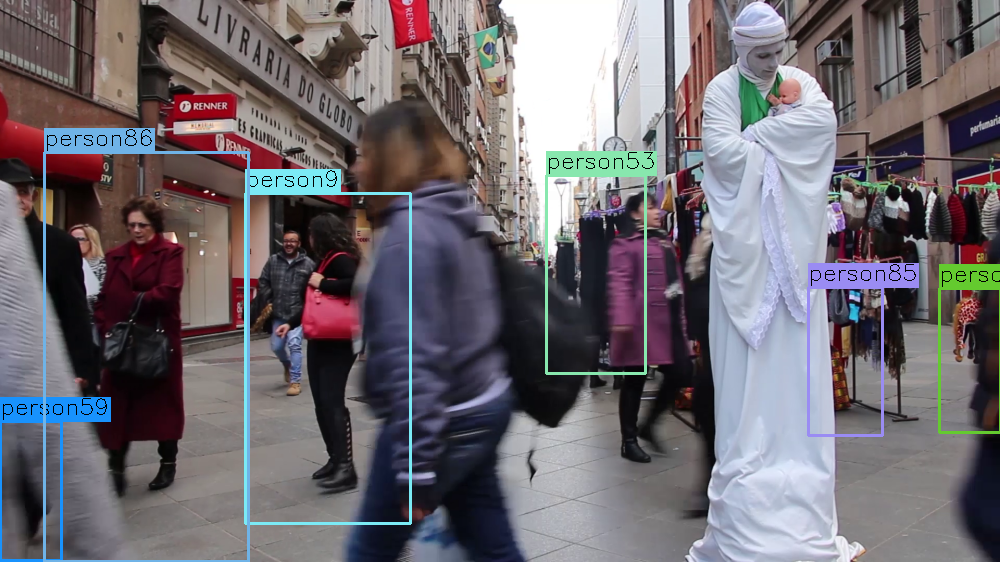
\includegraphics[width=\linewidth]{/home/luka/Workspaces/diplomski-rad/img/frame_26.png}
	\end{subfigure}
	\begin{subfigure}[b]{0.4\linewidth}
		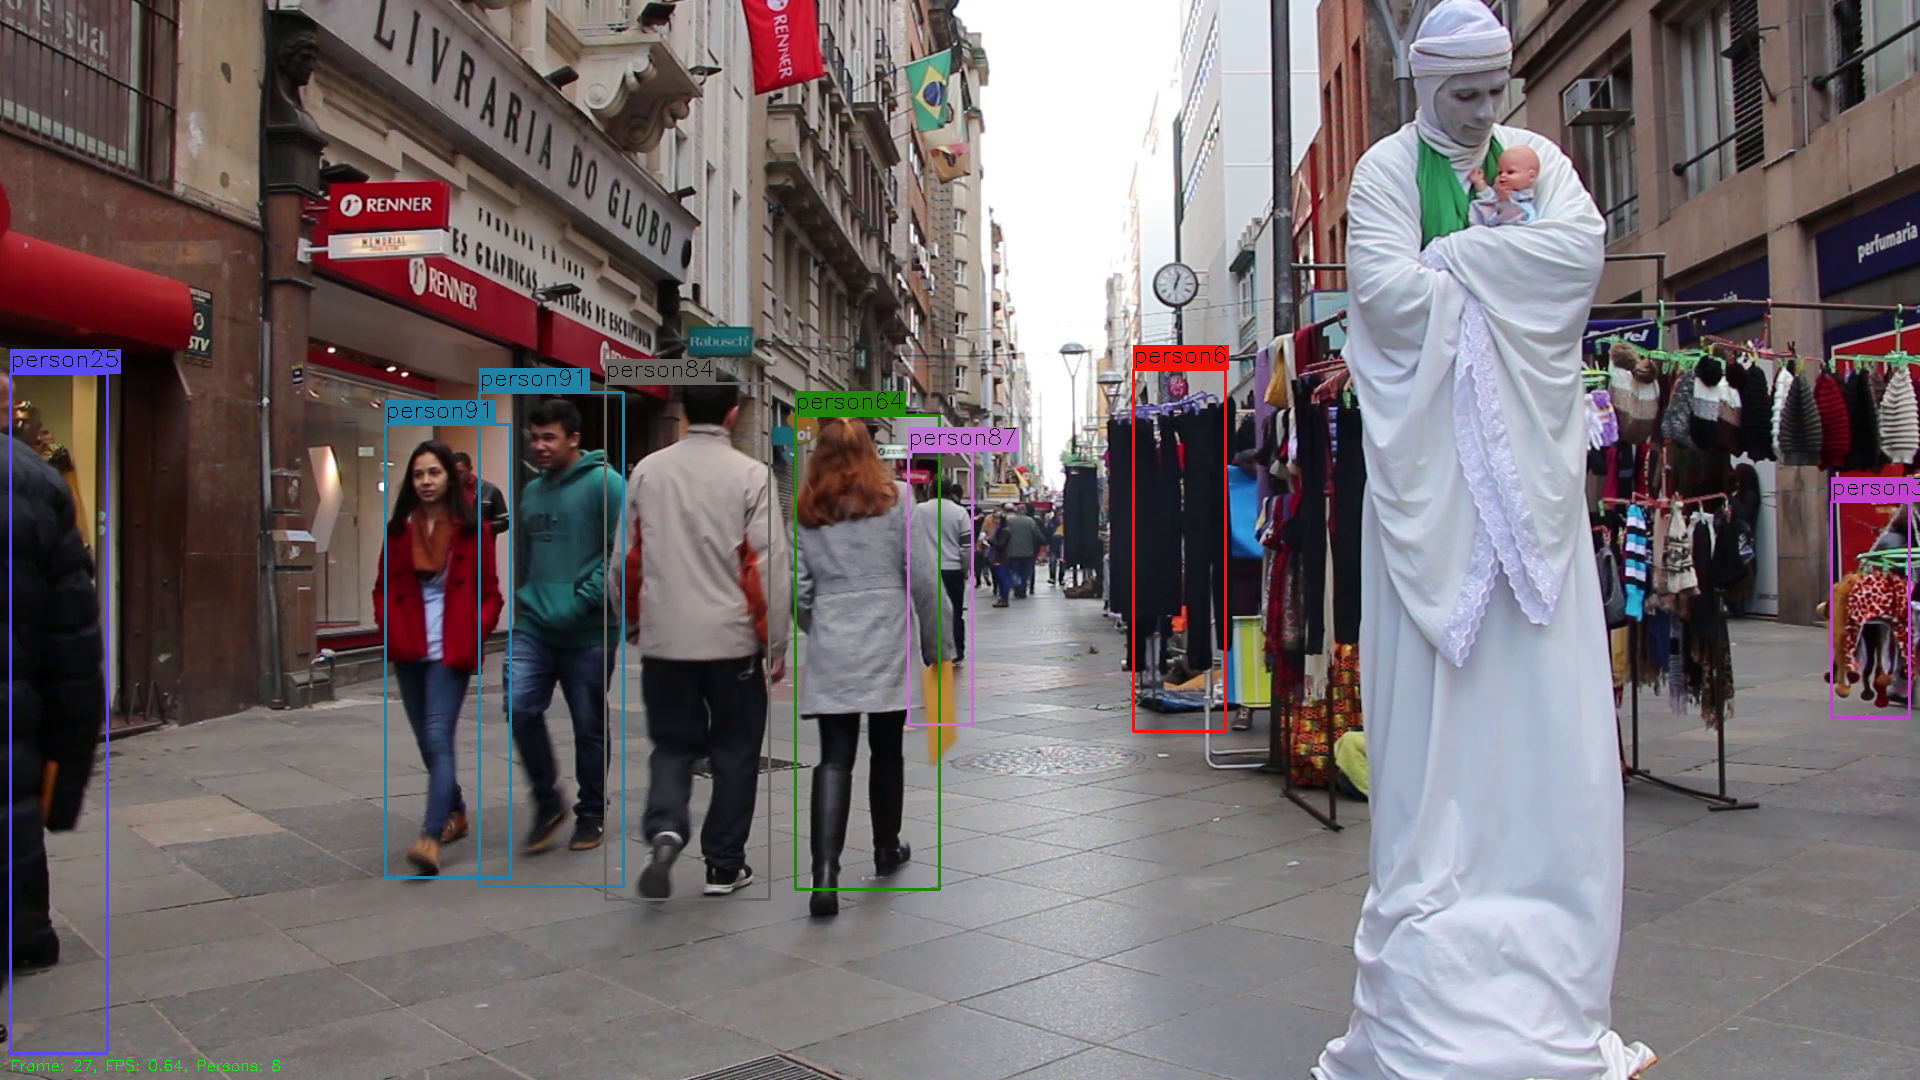
\includegraphics[width=\linewidth]{/home/luka/Workspaces/diplomski-rad/img/frame_27.png}
	\end{subfigure}
	\caption{Primjer konzistentnog praćenja osobe označene sa \textit{person87}}
	\label{img:tracking}
\end{figure}

\begin{figure}[htp]
	\centering
	\begin{subfigure}[b]{0.4\linewidth}
		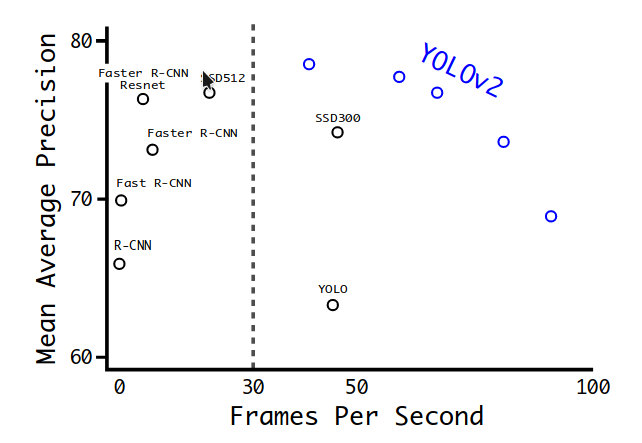
\includegraphics[width=\linewidth]{/home/luka/Workspaces/diplomski-rad/img/YoloGraph.png}
		\caption{Brzina i preciznost na skupu podataka VOC2007}
		\label{img:yolo_graph}
	\end{subfigure}
	\begin{subfigure}[b]{0.4\linewidth}
		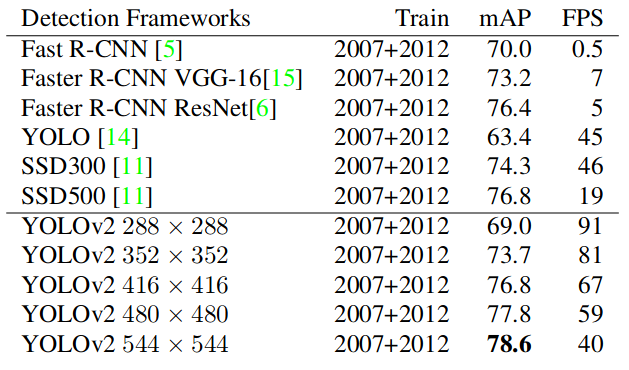
\includegraphics[width=\linewidth]{/home/luka/Workspaces/diplomski-rad/img/YoloTable.png}
		\caption{Usporedba raznih metoda za detekciju objekata}
		\label{img:yolo_table}
	\end{subfigure}
\caption{Rezultati YOLO algoritma}
\label{img:yolo_paper}
\end{figure}

Podaci sa slike \ref{img:yolo_graph} i \ref{img:yolo_table} preuzeti su iz rada \citep{YOLO}. Na slici \ref{img:yolo_table} vidljivo je nekoliko rezultata za YOLO algoritam. Jedina razlika između tih rezultata je veličina slike koja se dovodi na ulaz mreže. Logično, ako je ulaz manji, točnost je manja ali brzina je veća. Obrnuto, točnost je veća ali pod cijenu nešto sporijeg izvođenja. U ovom radu, istraživanje je provedeno na videu. Kako bi se izračunala točnost na ovom videu, kao i za Viola-Jones algoritam, računat je prosijek točnosti na spremljenim frameovima. Za YOLO to izgleda ovako:

\begin{table}[h]
\centering
\begin{tabular}{|rcl|}
\hline
	Broj vidljivih osoba po slici & & 5.67\\
\hline
	Broj detekcija po slici videa & & 5.16\\
\hline
	True Positivea po slici & & 4.53\\
\hline
	False Positivea po slici & & 0.32\\
\hline
	Preciznost (precision) & & 87.79\%\\
\hline
\end{tabular}
\caption{Razultati YOLO algoritma na videu Esquina Democratica}
\label{tab:Yolo_result}
\end{table}

Ovdje je točnost bolja nego u radu, ali stvar je u tome da je ovaj video izabran radi pračenja trajektorija te zato broj ljudi koji prolaze ulicom i nalaze se na slici nije toliko velik, samo 5.67 osoba po slici u prosjeku.

Video je zapravo niz slika pa se tada ovaj problem svodi na provođenje ovog algoritma za svaku sliku u videu (24 slike u sekundi). Kao što je već navedeno, u eksperimentima se algoritam izvodi na CPU, pa je stoga uvedena zastavica pri pozivu algoritma koja određuje koliko će slika u videu algoritam preskočiti prije nego uzme iduću sliku na obradu i predviđanje. Tako je moguće ubrzati izvođenje programa, te ako se osobe na slici kreću sporije, u nekoj koloni, moguće je, i čak poželjno, postaviti ovaj parametar na neki veći broj. Tada se standardni poziv programa u terminalu mijenja na sljedeći način:
\begin{center}
\begin{lstlisting}[language=Awk, caption=Poziv programa sa opcijom preskakanja zadanog broja (n) slika u videu]
python3 eval.py --skip_n_frames=n --video='path/to/video'
\end{lstlisting}
\end{center}

Podatak da su grafičke kartice za ove primjene 100 puta brže od procesora, daje podatak da bi se ovaj algoritam mogao izvršavati brzinom oko 25 FPS-a što je dovoljno i za video u stvarnom vremenu jer je standardna brzina videa 24 FPS-a. Dodatno, model se učita jednom i vrši se predikcija na svakoj slici sa tim, već učitanim, modelom. Dakle, prema tablici \ref{tab:img-performance} za predviđanje i postprocesiranje slike dovoljno je oko 1.2 sekunde po slici što daje brzinu od oko 80 FPS-a na grafičkoj kartici, što je vrlo blizu originalnog rada. Ova brzina postignuta je jer se u pozadini Kerasa izvodi Tensorflow koji je maksimalno optimiziran i koristi biblioteke kao što su NumPy i SciPy koje su napisane u C-u. 

Nadalje, u poglavlju o implementaciji algoritma YOLO, bilo je govora o Non-Maximal Suppression metodi koju ovaj algoritam koristi za predviđanje i evaluaciju kako bi maknuo redundantne okvire. No, tamo je naveden prag pouzdanosti koji utječe na to koji od okvira uopće dolaze u obzir pri predviđanju objekata. Taj prag je također parametar koji je moguće mijenjati. Naravno, tako će algoritam prikazivati sve više šuma, te je stoga potrebno dobro istražiti kako se algoritam ponaša na danom skupu podataka. Na slici \ref{img:threshold-impact} prokazana je ekstremna situacija kada se ovaj prag postavi na vrijednost $0$ kada algoritam isctrava sve okvire. U ovoj implementaciji, konkretno, prag je izabran eksperimentalno i postavljen na 0.3. Ako korisnik želi postaviti neki drugi prag, to mora biti broj između $0$ i $1$. Korištenje ove zastavice omogućeno je sljedećom naredbom:
\begin{center}
\begin{lstlisting}[language=Awk, caption=Poziv programa sa prozvoljnim pragom pouzdanosti okvira]
python3 eval.py --threshold=n --video='path/to/video'
\end{lstlisting}
\end{center}

\begin{figure}[htp]
	\centering
	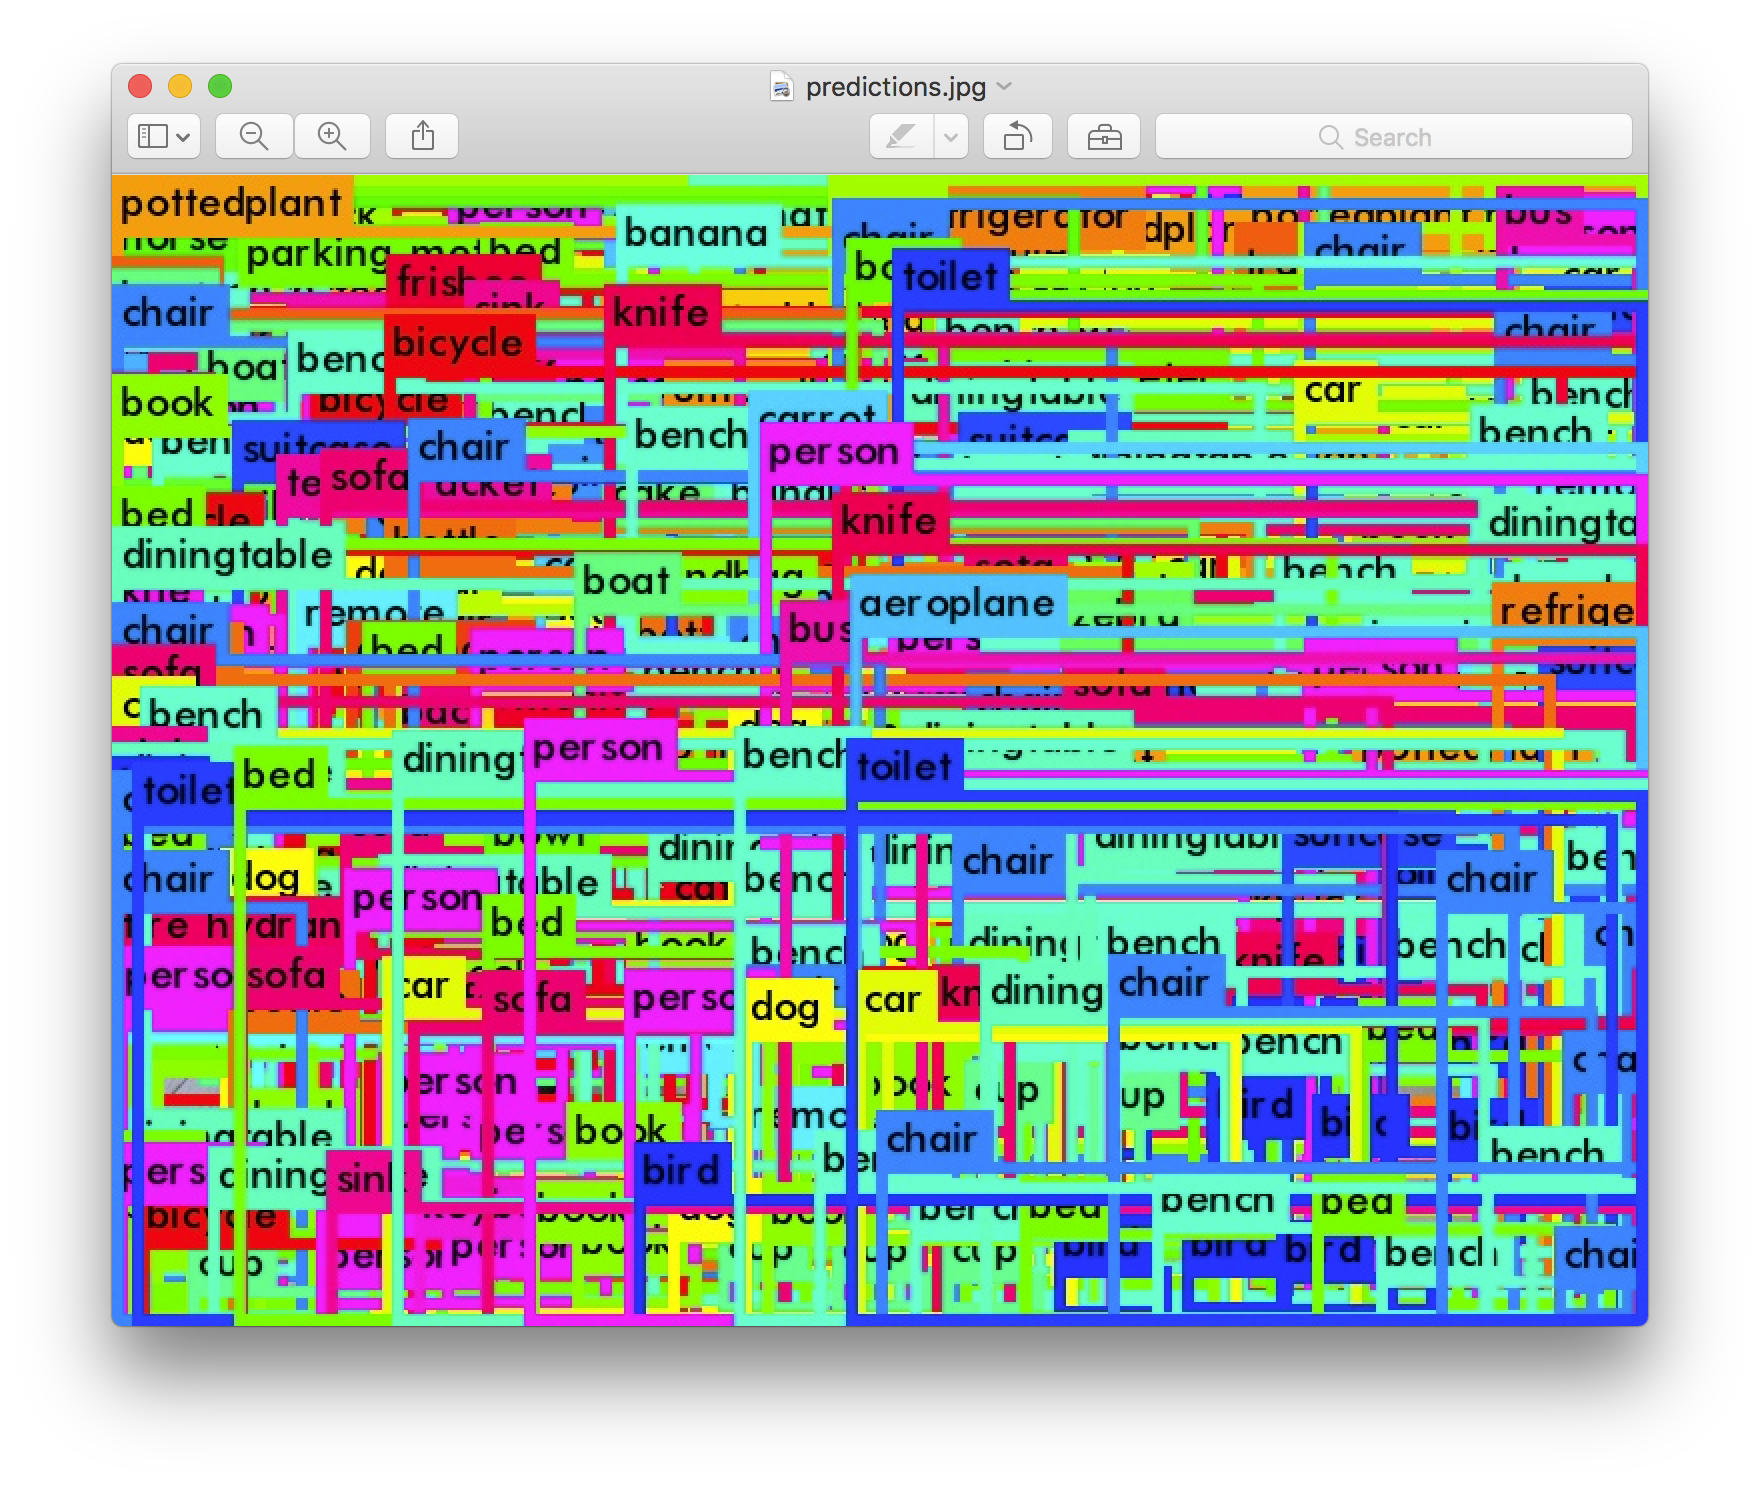
\includegraphics[width=8cm]{/home/luka/Workspaces/diplomski-rad/img/threshold_impact.png}
	\caption{Rezultat ako se preg postavi na vrijednost 0 \citep{YOLO}}
	\label{img:threshold-impact}
\end{figure}

\bigskip
Ovime je završen zadatak detekcije objekata (klasifikacija i lokalizacija). Dinamičnost videa u odnosu na sliku donosi sa sobom još jedan problem, a to je praćenje kretanja objekata. 
\bigskip

Ovaj zadatak može biti riješen na više načina, no u ovoj implementaciji odabrana je već spomenuta metoda \textit{Intersection over Union}. Ova metoda prati trajektorije objekata na način da zapamti predviđene okvire iz prošle slike (\textit{engl. frame}) te nakon predviđanja okvira iduće slike iterira kroz okvire nove slike i uspoređuje ih sa svim okvirima prošle slike. Tada okvir iz nove slike koji ima najveći IoU rezultat sa okvirom stare slike, postaje taj okvir. To se manifestira u videu na način da novi okvir preuzme boju okvira sa prošle slike s kojim ima najveće poklapanje. Ova metoda, kao i sve druge, ima i svojih nedostataka. Primjerice, ako je okvir objekta sa prošle slike imao vrlo malo preklapanje sa okvirom potpuno drugog objekta sa nove slike, a okvir sa nove slike nema doticaja sa nijednim drugim okvirom sa stare slike, preuzet će boju okvira sa stare slike. Situacija je prikazana slikom \ref{img:trajectories1} To je neželjeno ponašanje jer to nije taj objekt. To je riješeno na način da svaki okvir, pri stvaranju (predviđanju) dobija neku svoju nasumičnu boju. Zatim, kada dođe do gore opisane situacije, gleda se rezultat IoU metode te se stavlja prag, odnosno, postotak preklapanja, za koji možemo reći da je dovoljan da odredimo da je to isti objekt iz prošle slike. U implementaciji je taj prag postavljen na vrijednost $0.5$. 

\begin{figure}[htp]
	\centering
	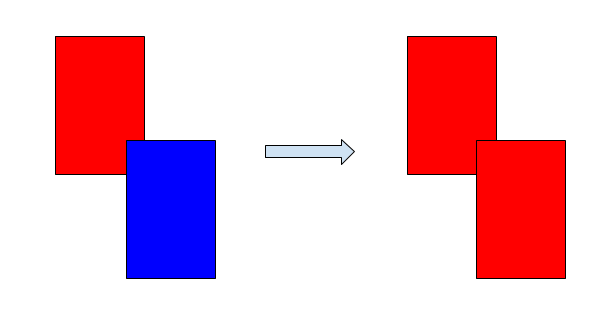
\includegraphics[width=10cm]{/home/luka/Workspaces/diplomski-rad/img/Trajectories.png}
	\caption{Situacija kada okvir novog objekta preuzme boju starog objekta na temelju zanemarivo malog poklapanja}
	\label{img:trajectories1}
\end{figure}

Jedan od primjera takvih pogrešaka prikazan je na slici \ref{img:err-trajectories}. Vidi se da na prvoj slici u lijevom rubu slike, postoje dvije osobe: \textit{person10} i \textit{person69}. Na idućoj slici, viljivo je da je algoritam promijenio ime osobe 69 u osobu 10. To se događa jer se promijenila veličina okvira te sada okvir osobe 69 ima veći IoU sa osobom 10 iz prethodnog okvira nego sa osobom 69.

\begin{figure}[htp]
	\centering
	\begin{subfigure}[b]{0.4\linewidth}
		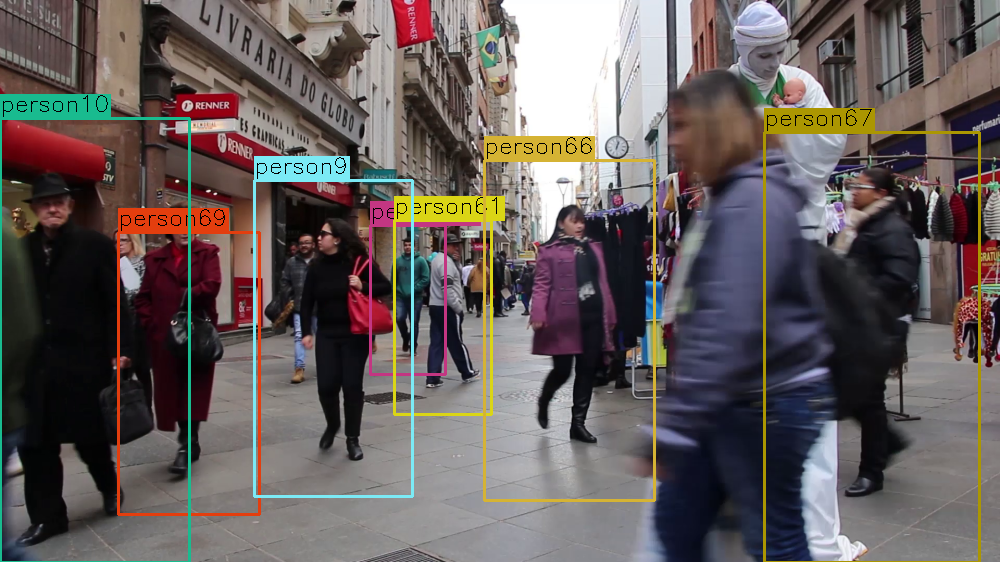
\includegraphics[width=\linewidth]{/home/luka/Workspaces/diplomski-rad/img/frame_8.png}
	\end{subfigure}
	\begin{subfigure}[b]{0.4\linewidth}
		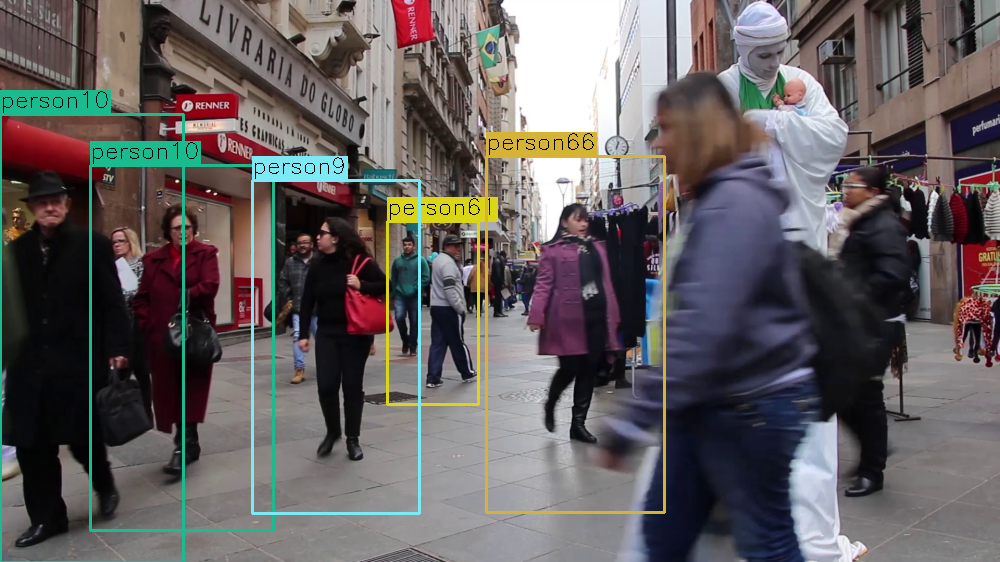
\includegraphics[width=\linewidth]{/home/luka/Workspaces/diplomski-rad/img/frame_9.png}
	\end{subfigure}
	\caption{Primjer pogreške kod praćenja trajektorija metodom IoU}
	\label{img:err-trajectories}
\end{figure}

Kod ove metode javlja se još jedan problem, a to je da ako se objekt kreće uz objektiv kamere i ide slijeva nadesno ili obrnuto, svi okviri konvergiraju u okvir tog objekta. Ovaj problem se javlja zbog načina računanja trajektorija objekta metodom IoU. Kada objekt prođe ispred objektiva, njegov okvir je jako velik, gotovo kao cijeli objektiv. Kada se u tom koraku računa trajktorija ostalih objekata, svi ostali okviri imaju najveći IoU sa tim okvirom te se algoritam dalje ponaša kao da su svi oni ista osoba. Ovaj problem riješen je na način da je postavljen prag veličine okvira koji se crta. Što je objekt bliže objektivu, on je veći, pa je na ovaj način odabrana blizina objekata koji se detektiraju. U implementaciji je ovaj prag postavljen na vrijednost od $100000$.

\begin{figure}[htp]
	\centering
	\begin{subfigure}[b]{0.4\linewidth}
		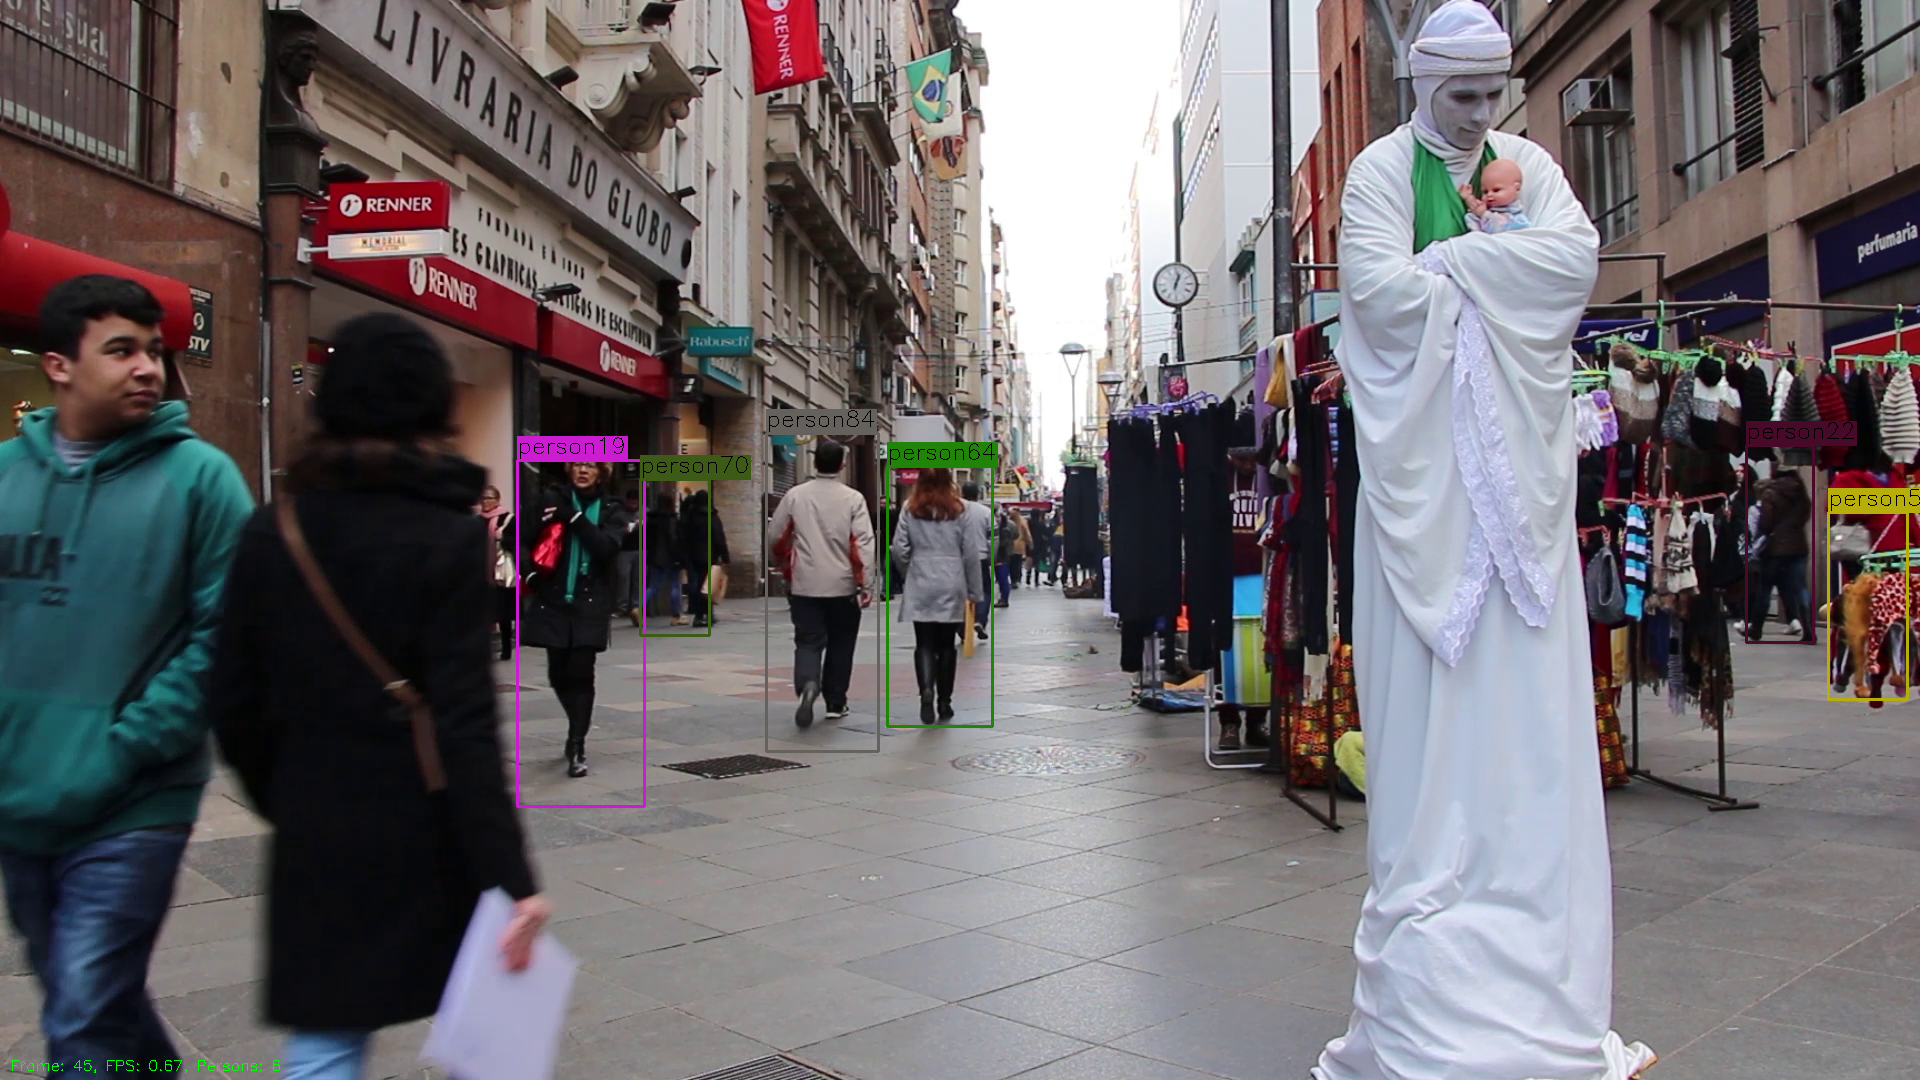
\includegraphics[width=\linewidth]{/home/luka/Workspaces/diplomski-rad/img/frame_45.png}
	\end{subfigure}
	\begin{subfigure}[b]{0.4\linewidth}
		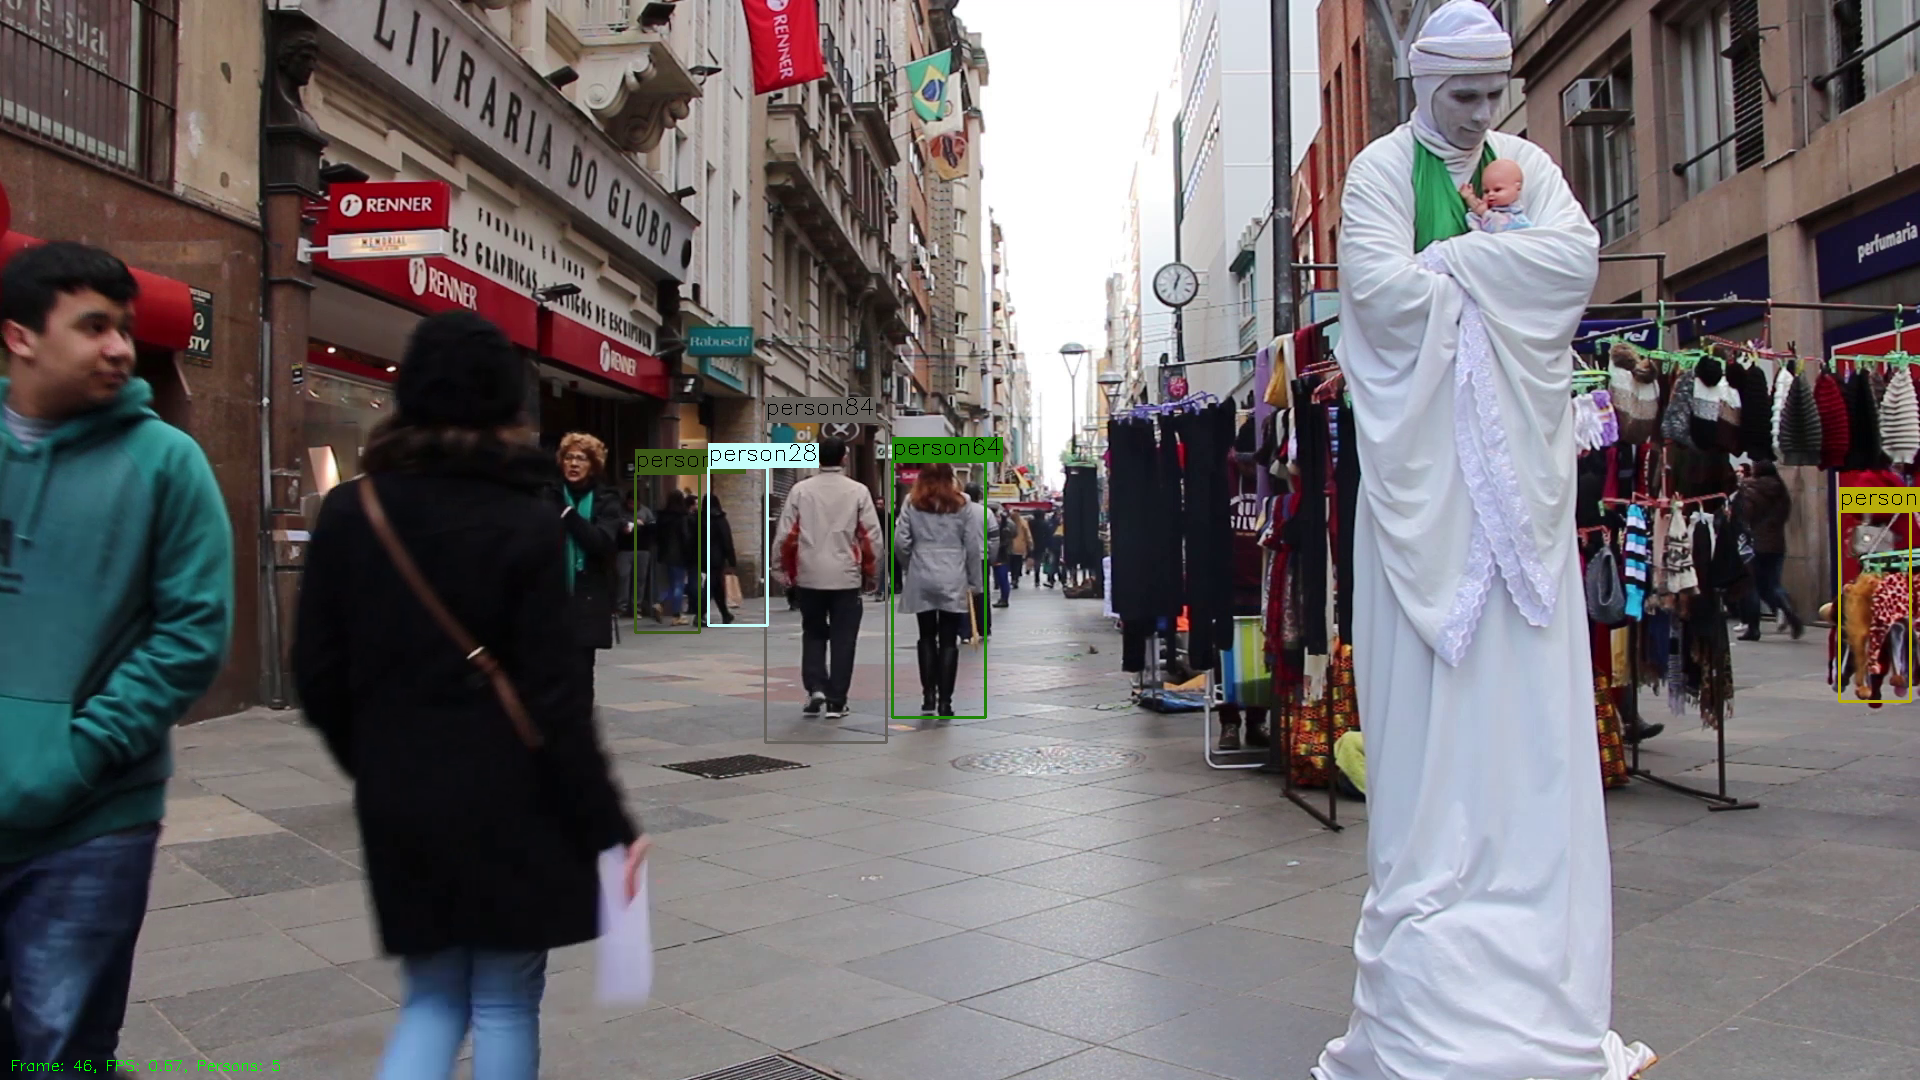
\includegraphics[width=\linewidth]{/home/luka/Workspaces/diplomski-rad/img/frame_46.png}
	\end{subfigure}
	\begin{subfigure}[b]{0.4\linewidth}
		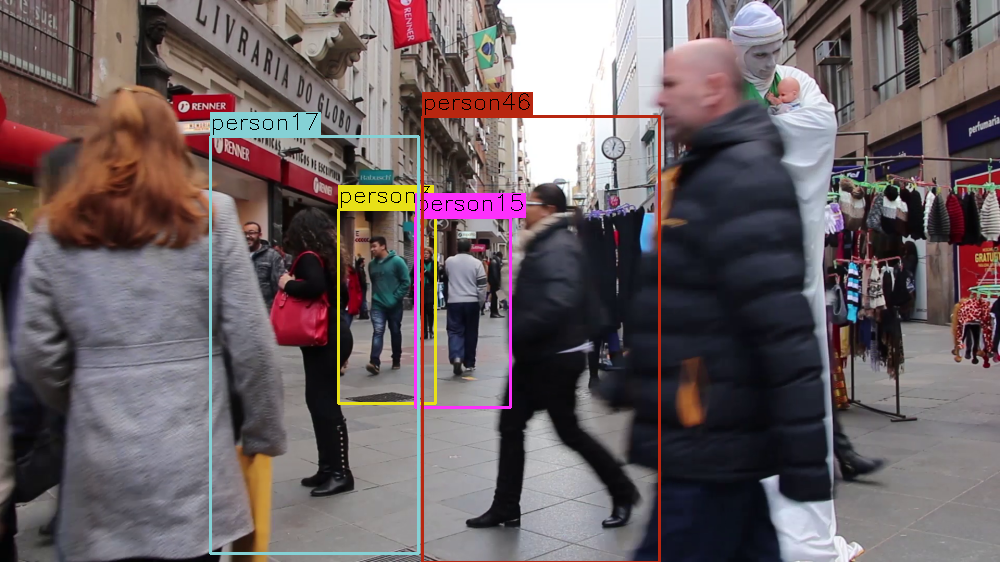
\includegraphics[width=\linewidth]{/home/luka/Workspaces/diplomski-rad/img/frame_47.png}
	\end{subfigure}
	\begin{subfigure}[b]{0.4\linewidth}
		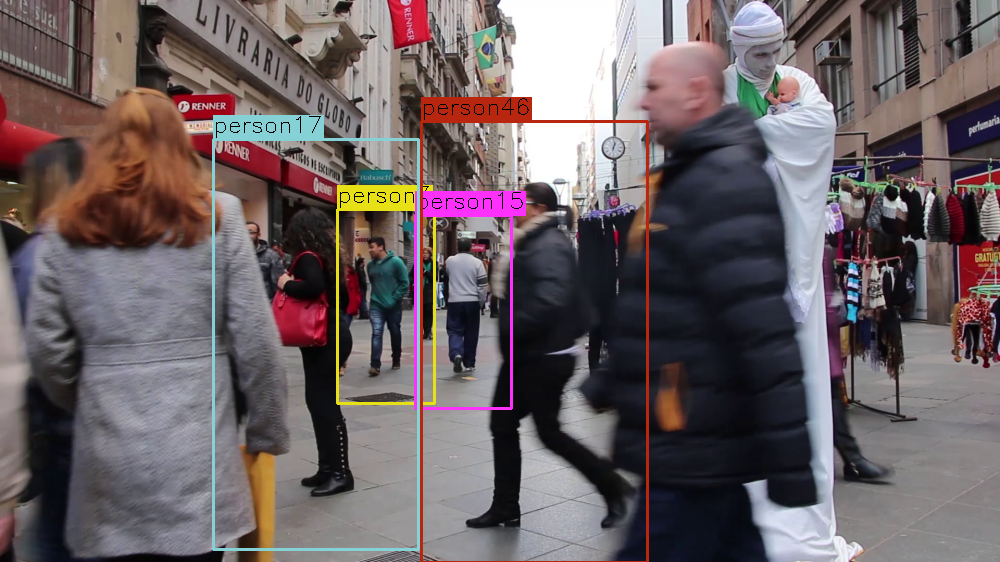
\includegraphics[width=\linewidth]{/home/luka/Workspaces/diplomski-rad/img/frame_48.png}
	\end{subfigure}
	\caption{Primjer kretanja objekta uz objektiv kamere}
	\label{img:close-objective}
\end{figure}